\pdfoutput=1
\pdfcompresslevel=9
\pdfinfo
{
    /Author (Łukasz Rafał Szewczyk)
    /Title (Projekt i~implementacja biblioteki dla Qt i~Qt~Quick do operowania na wykresach typu biurowego)
    /Subject (Tematyka)
    /Keywords (Slowa kluczowe)
}
%\documentclass[a4paper,polish,onecolumn,oneside,floatssmall,11pt,titleauthor,wide,openright]{mwrep}
%\usepackage[scale={0.7,0.8},paper=a4paper,twoside]{geometry}
\documentclass[a4paper,onecolumn,oneside,11pt,wide,floatssmall]{mwrep}
% \usepackage{polish}
\usepackage{mathtools}
\usepackage{amsfonts}
\usepackage{amssymb}
\usepackage{amsthm}
\usepackage{bookman}
\usepackage{float}
\usepackage{enumerate}

\usepackage{geometry}
\usepackage[utf8x]{inputenc}
\usepackage[T1]{fontenc}
% \usepackage{t1enc}
% \usepackage[pdftex, bookmarks]{hyperref}
\usepackage[pdftex, bookmarks=false]{hyperref}
\def\url#1{{ \tt #1}}

\usepackage{listings}
\usepackage{eurosym}
% marginesy
\textwidth\paperwidth
\advance\textwidth -55mm
\oddsidemargin-0.9in
\advance\oddsidemargin 33mm
\evensidemargin-0.9in
\advance\evensidemargin 33mm
\topmargin -1in
\advance\topmargin 25mm
\setlength\textheight{48\baselineskip}
\addtolength\textheight{\topskip}
\marginparwidth15mm

\clubpenalty=10000 % to kara za sierotki
\widowpenalty=10000 % nie pozostawia wdów
\brokenpenalty=10000 % nie dzieli wyrazów pomiędzy stronami
\sloppy

\tolerance4500
\pretolerance250
\hfuzz=1.5pt
\hbadness1450

% ŻYWA PAGINA
\renewcommand{\chaptermark}[1]{\markboth{\scshape\small\bfseries \
#1}{\small\bfseries \ #1}}
\renewcommand{\sectionmark}[1]{\markboth{\scshape\small\bfseries\thesection.\
#1}{\small\bfseries\thesection.\ #1}}
\newcommand{\headrulewidth}{0.5pt}
\newcommand{\footrulewidth}{0.pt}
\pagestyle{uheadings}

\usepackage[pdftex]{color,graphicx}
\usepackage[polish]{babel}

% \textheight232mm
% \setlength{\textwidth}{\textwidth}
% \setlength{\oddsidemargin}{\evensidemargin}
% \setlength{\evensidemargin}{0.3cm}
\usepackage[sort, compress]{cite}

%\usepackage{multibib}
%\newcites{bk,st,doc,web}{Książki i~artykuły,Standardy i~zalecenia,Dokumentacja produktów,Publikacje i~serwisy internetowe}

\theoremstyle{definition}
\newtheorem{defn}{Definicja}[section]
\newtheorem{conj}{Teza}[section]
\newtheorem{conjmain}{Teza}
\newtheorem{exmp}{Przykład}[section]

\theoremstyle{plain}% default
\newtheorem{thm}{Twierdzenie}[section]
\newtheorem{lem}[thm]{Lemat}
\newtheorem{prop}[thm]{Hipoteza}
\newtheorem*{cor}{Wniosek}

\theoremstyle{remark}
\newtheorem*{rem}{Uwaga}
\newtheorem*{note}{Uwaga}
\newtheorem{case}{Przypadek}

\definecolor{ListingBackground}{rgb}{0.95,0.95,0.95}

\begin{document}

% kody źródłowe wplatane w tekst
\lstdefinestyle{incode}
{
basicstyle={\footnotesize},
keywordstyle={\bf\footnotesize\color{blue}},
commentstyle={\em\footnotesize\color{magenta}},
numbers=left,
stepnumber=5,
firstnumber=1,
numberfirstline=true,
numberblanklines=true,
numberstyle={\sf\tiny},
numbersep=10pt,
tabsize=2,
xleftmargin=17pt,
framexleftmargin=3pt,
framexbottommargin=2pt,
framextopmargin=2pt,
framexrightmargin=0pt,
showstringspaces=true,
backgroundcolor={\color{ListingBackground}},
extendedchars=true,
% title=\lstname,
captionpos=b,
% abovecaptionskip=1pt,
% belowcaptionskip=1pt,
frame=tb,
framerule=0pt,
}

% kody źródłowe z podpisem
\lstdefinestyle{outcode}
{
basicstyle={\footnotesize},
keywordstyle={\bf\footnotesize\color{blue}},
commentstyle={\em\footnotesize\color{magenta}},
numbers=left,
stepnumber=5,
firstnumber=1,
numberfirstline=true,
numberblanklines=true,
numberstyle={\sf\tiny},
numbersep=10pt,
tabsize=2,
xleftmargin=17pt,
framexleftmargin=3pt,
framexbottommargin=2pt,
framextopmargin=2pt,
framexrightmargin=0pt,
showstringspaces=true,
backgroundcolor={\color{ListingBackground}},
extendedchars=true,
% title=\lstname,
captionpos=b,
% abovecaptionskip=1pt,
% belowcaptionskip=1pt,
frame=tb,
framerule=0.1pt,
}

\renewcommand*\lstlistingname{Wydruk}
\renewcommand*\lstlistlistingname{Spis wydruków}

\pagenumbering{roman}
\renewcommand{\baselinestretch}{1.0}
\raggedbottom

\begin{titlepage}
    % Strona tytułowa
    \vbox to\textheight{\hyphenpenalty=10000
    \begin{center}
	\begin{tabular}{p{107mm} p{9cm}}
	    \begin{minipage}{9cm}
	      \begin{center}
	      Politechnika Warszawska \\
	      Wydział Elektroniki i~Technik Informacyjnych \\
	      Instytut Informatyki
	      \end{center}
	    \end{minipage}
	    &
	    \begin{minipage}{8cm}
	    \begin{flushleft}
	     \footnotesize
	      Rok akademicki 2012/2013
	    \vspace*{2.75\baselineskip}
	    \end{flushleft}
	    \end{minipage} \\
	\end{tabular}
	\vspace*{3.75\baselineskip}
	\par\vspace{\smallskipamount}
	\vspace*{2\baselineskip}{\LARGE Praca dyplomowa inżynierska\par}
	\vspace{3\baselineskip}{\LARGE\strut Łukasz Rafał Szewczyk\par}
	\vspace*{2\baselineskip}{\huge\bfseries Projekt i~implementacja biblioteki dla Qt i~Qt~Quick do operowania na wykresach typu biurowego\par}

	\vspace*{7\baselineskip}
	\hfill\mbox{}\par\vspace*{\baselineskip}\noindent
	\begin{tabular}[b]{@{}p{3cm}@{\ }l@{}}
	    {\large\hfill } & {\large }
	\end{tabular}
	\hfill
	\begin{tabular}[b]{@{}l@{}}
	Opiekun pracy: \\[\smallskipamount]
	{\large mgr inż. Witold Wysota}
	\end{tabular}\par
	\vspace*{4\baselineskip}
    \begin{tabular}{p{\textwidth}}
    \begin{flushleft}
	\begin{minipage}{7cm}
	Ocena \dotfill
	\par\vspace{1.6\baselineskip}
	\dotfill
	\par\noindent
	\centerline{\footnotesize Podpis Przewodniczącego} \par
	\centerline{\footnotesize Komisji Egzaminu Dyplomowego}\par
	\end{minipage}
    \end{flushleft}
    \end{tabular}
    \end{center}}

    % Życiorys
    \newpage\thispagestyle{empty}
    \begin{tabular}{p{5cm} p{12cm}}
    \begin{minipage}{5cm}
    \center
    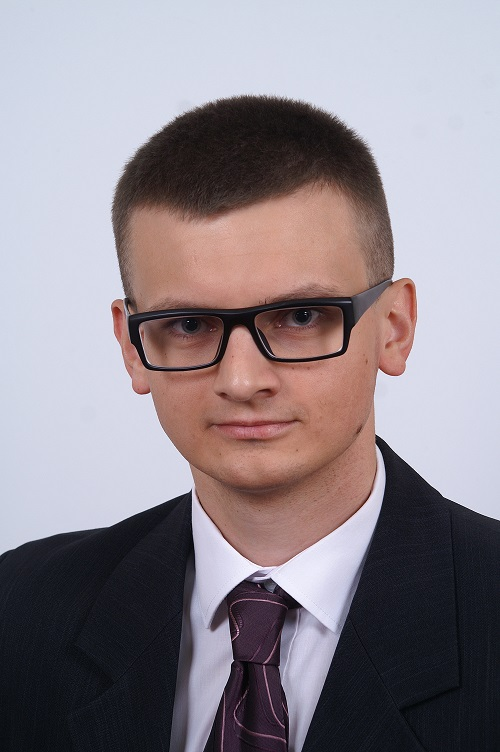
\includegraphics[height=6.5cm,width=4.5cm]{img/foto.jpg}
    \end{minipage}
    &
    \begin{minipage}{12cm}
    \begin{flushleft}
    \par\noindent\vspace{1\baselineskip}
    \begin{tabular}[h]{l l}
    {\normalsize\it Specjalność:} & Informatyka -- \\
    & Inżynieria systemów informatycznych
    \end{tabular}
    \par\noindent\vspace{1\baselineskip}
    \begin{tabular}[h]{l l}
    {\normalsize\it Data urodzenia:} & {\normalsize 02 grudnia 1990~r.}
    \end{tabular}
    \par\noindent\vspace{1\baselineskip}
    \begin{tabular}[h]{l l}
    {\normalsize\it Data rozpoczęcia studiów:} & {\normalsize 1 października 2009 r.}
    \end{tabular}
    \par\noindent\vspace{1\baselineskip}
    \end{flushleft}
    \end{minipage}
    \end{tabular}
    \vspace*{1\baselineskip}
    \begin{center}
	{\large\bfseries Życiorys}\par\bigskip
    \end{center}

    \indent
    Urodziłem się dnia 2. grudnia 1990 roku w~Warszawie. Całe dotychczasowe życie spędziłem mieszkając w~podwarszawskiej Kobyłce, w~której to uczęszczałem do szkoły podstawowej i~gimnazjum. Z~powodu zainteresowania matematyką zdecydowałem się w~roku 2006 rozpocząć naukę w~XVIII Liceum Ogólnokształcącym im. Jana Zamoyskiego w~Warszawie, w~klasie o~profilu matematyczno-fizyczno-informatycznym. W~pierwszej klasie liceum rozpocząłem równiez swoją przygodę z~siatkówką w~klubie Junior Stolarka Wołomin.
    \par
Dobre wyniki osiągnięte na egzaminach maturalnych w~roku 2009 pozwoliły mi dostać się na dzienne studia inżynierskie na Wydziale Elektroniki i Technik Informacyjnych Politechniki Warszawskiej.
W~trakcie studiów poza nauką kontynuowałem swój siatkarski rozwój, dzięki czemu trafiłem do zespołu AZS Politechnika Warszawska, który reprezentowałem w~rozgrywkach Młodej Ligi, przeznaczonych dla zawodników poniżej 23 roku życia, oraz w~rozgrywkach akademickich. W~2012 roku wróciłem do swojego macierzystego klubu, który w~międzyczasie wrócił do swojej historycznej nazwy -- Huragan Wołomin. W~sezonie 2012/13 udało mi się wywalczyć z~tym klubem awans do II ligi siatkówki.


    \par
    \vspace{2\baselineskip}
    \hfill\parbox{15em}{{\small\dotfill}\\[-.3ex]
    \centerline{\footnotesize podpis studenta}}\par
    \vspace{3\baselineskip}
    \begin{center}
 	{\large\bfseries Egzamin dyplomowy} \par\bigskip\bigskip
    \end{center}
    \par\noindent\vspace{1.5\baselineskip}
    Złożył egzamin dyplomowy w dn. \dotfill
    \par\noindent\vspace{1.5\baselineskip}
    Z wynikiem \dotfill
    \par\noindent\vspace{1.5\baselineskip}
    Ogólny wynik studiów \dotfill
    \par\noindent\vspace{1.5\baselineskip}
    Dodatkowe wnioski i uwagi Komisji \dotfill
    \par\noindent\vspace{1.5\baselineskip}
    \dotfill

    % Streszczenie
    \newpage\thispagestyle{empty}
    \vspace*{2\baselineskip}
    \begin{center}
	{\large\bfseries Streszczenie}\par\bigskip
    \end{center}

    {\itshape
    Praca prezentuje projekt biblioteki zawierającej uniwersalny silnik służący do tworzenia  biurowych wykresów w~Qt oraz Qt~Quick. Wykresy te są w~szczególności nastawione na interakcję z~użytkownikiem oraz współpracę z~już istniejącymi mechanizmami Qt.
	W~ramach pracy wykonano opis i~analizę wymagań oraz projekt architektury biblioteki. Zaplanowano również testy tworzonej biblioteki. Projekt zakłada implementację z~wykorzystaniem języka C++ oraz bibliotek Qt w~wersji 5.
	}
    \vspace*{1\baselineskip}

    \noindent{\bf Słowa kluczowe}: {\itshape uniwersalny silnik wykresów, obiektowa architektura.}
    \par
    \vspace{4\baselineskip}
    \begin{center}
	{\large\bfseries Abstract}\par\bigskip
    \end{center}
    \noindent{\bf Title}: {\itshape Project and implementation of office type charts library for Qt and Qt Quick}\par
    \vspace*{1\baselineskip}
    {\itshape
    This paper presents a~project of library containing universal engine for creating office charts in Qt and Qt~Quick. These plots are particularly focused on the user interaction and collaboration with existing mechanisms in Qt.
The paper contains description and~analysis of requirements and project of architecture of library. Also planned tests of designed library. The project involves the implementation using C++ language and Qt libraries in version 5.}
    \vspace*{1\baselineskip}

    \noindent{\bf Key words}: {\itshape universal charting engine, object oriented architecture.}

\end{titlepage}

% ex: set tabstop=4 shiftwidth=4 softtabstop=4 noexpandtab fileformat=unix filetype=tex spelllang=pl,en spell:


\tableofcontents
% \addcontentsline{toc}{chapter}{{Przedmowa1}{vii}}{vii}

% \chapter*{Spis tablic, rysunków i~wydruków}
% \listoftables
% \listoffigures
% \lstlistoflistings

%\setlength{\baselineskip}{7mm}
\newpage
\pagenumbering{arabic}
\setcounter{page}{1}

\chapter*{Wstęp}
Częstym zadaniem tworzonego oprogramowania jest prezentacja pewnych danych. Nawet najlepszy program wykonujący skomplikowane obliczenia jest niewiele wart dla klienta, jeśli nie potrafi w~przystępny sposób zaprezentować efektów swoich działań.
 
Jedną z~podstawowych form prezentacji danych w~informatyce (i~nie tylko) jest tabela, która umożliwia wyświetlanie danych z~dużą precyzją. Qt posiada już architekturę służącą tworzeniu takich systemów -- Model-Widok~\cite{Qt:Model:View}. Jest to bardzo popularna platforma umożliwiająca tworzenie skomplikowanych interaktywnych tabelek prezentujących dane z~różnych źródeł, m.in. z~bazy danych.

Inną formą prezentacji danych są wykresy, których popularność jest porównywalna do tabel. Jest to forma dużo bardziej przystępna dla ludzkiej percepcji. Ułatwiają szybkie porównywanie wielu rekordów oraz wyznaczanie tendencji. Ponadto ich obrazkowa natura oraz możliwe animacje sprawiają, że jest to forma bardzo atrakcyjna dla końcowego użytkownika oprogramowania.
%Qt posiada już kilka bibliotek służących tworzeniu wykresów, jednak nadal istnieje zapotrzebowanie na wartościowe rozwiązanie open-source, co wykazuję w~rozdziale \textit{Przegląd dziedziny}.

W ostatnich latach da się zauważyć wyraźną tendencję odchodzenia od tabel na rzecz graficznych form prezentacji danych. Tendencja ta jest szczególnie nasilona w~sektorze urządzeń mobilnych, takich jak telefony klasy smartphone. Dodatkowo rozpowszechnienie się technologii ekranów dotykowych umożliwia realizację interakcji na niedostępnym dotychczas poziomie. Qt od wersji 5.2 ma być dostępne na najpopularniejszych tego typu urządzaniach pracujących pod kontrolą systemów Android oraz iOS. 

Co prawda Qt posiada już kilka bibliotek umożliwiających tworzenie wykresów, jednak brakuje darmowych, gotowych do użycia rozwiązań umożliwiających interaktywną prezentację danych. Dodatkowo nowa technologia tworzenie interfejsów użytkownika -- Qt~Quick cierpi na niedobór bibliotek dostarczających komponentów wyższego poziomu. Jest to odpowiedni moment na wprowadzenie na rynek produktu, który ma szansę zyskać dużą popularność, choćby z~powodu braku konkurencji.

Moja praca inżynierska składa się z~rozdziałów opisujących kolejne etapy tworzenia biblioteki. W~rozdziale~\ref{chap:przeglad} omawiam dostępne biblioteki do tworzenia wykresów w~Qt, następnie przedstawiam opis i~analizę wymagań stawianych mojej bibliotece. Kolejny rozdział to inżynierski projekt architektury całej biblioteki. Następne dwa rozdziały są poświęcone implementacji oraz testom biblioteki. Ostatni  zawiera wnioski dotyczące stworzonej biblioteki oraz możliwości jej dalszego rozwoju. 

\chapter{Wprowadzenie}
W~tym rozdziale przedstawiam podstawy Qt oraz Qt~Quick, dzięki którym dowolny czytelnik powinien zrozumieć zawartość mojej pracy. Następnie opisuję podstawowe założenia, cele oraz cechy stworzonej biblioteki.

\section{Qt}
Qt jest zbiorem bibliotek języka C++, które są dostępne na licencjach LGPL, GPL oraz komercyjnej. Lista bibliotek jest dość okazała, a~znaleźć na niej można narzędzia do tworzenia interfejsów użytkownika, parsowania plików XML czy dostępu do baz danych. Naczelną zasadą Qt jest: \textit{pisz raz, kompiluj wielokrotnie}~\footnote{\url{http://qt-project.org/wiki/QtWhitepaper}} -- dzięki takiemu podejściu programy napisane w~Qt są przenośne pomiędzy najpopularniejszymi platformami na poziomie kodu źródłowego.  

Najnowsza dostępna wersja Qt to 5.1. Nowa odsłona dostarcza programistom szereg usprawnień oraz modułów, m.in. do obsługi formatu JSON. Jednak głównym punktem Qt~5 jest nowa implementacja Qt~Quick. 

Do implementacji Qt~Quick~2 wykorzystano OpenGL i~SceneGraph, co znacznie poprawiło wydajność tego systemu. Qt~5 rozpoczęło też nowy kierunek rozwoju aplikacji wykorzystujących Qt. Qt~Quick jest promowany jako zalecany sposób tworzenia interfejsów użytkownika. Docelowo aplikacje Qt mają być podzielone na GUI napisane w~QML oraz logikę zaprogramowaną w~C++.

\subsection{Narzędzia}
Najważniejszymi narzędziami, które umożliwiają tudzież ułatwiają pracę z~Qt są:
\begin{itemize}
\item moc (Meta Object Compiler) -- specjalny program, który można porównać do preprocesora. Na podstawie naszego kodu generuje on dodatkowe pliki źródłowe potrzebne Qt, niewidoczne dla programisty.
\item uic (User Interface Compiler) -- kompilator plików *.ui, które zawierają informację o~układzie interfejsu użytkownika.
\item qmake -- program ułatwiający zarządzanie procesem budowania projektu.
\item Qt Creator -- zintergrowane środowisko programistyczne, przeznaczone głównie dla języków C++, QML i~JavaScript.
\item Qt Designer -- program umożliwiający łatwe tworzenie interfejsów użytkownika. Generuje on wspomniane juz pliki *.ui.
\end{itemize}


\subsection{QObject}
C++ nie wymusza dziedziczenia po określonej klasie, jak ma to miejsce chociażby w~Javie, gdzie zawsze na szczycie drzewa dziedziczenia znajduje się klasa \textit{Object}. Qt wprowadza swoją klasę -- \textit{QObject}. Dzięki wielodziedziczeniu, nie musimy rezygnować z dotychczasowej hierarchii dziedziczenia, aby otrzymać wiele ciekawych możliwości płynących z~wykorzystania \textit{QObject}.
Niektóre z~nich to:
\begin{itemize}
\item Relacja rodzic--dziecko, która jest nawiązywana w chwili tworzenia obiektów. Umożliwia ona wyszukiwanie dzieci danego obiektu po ich klasie, bądź nazwie. Ponadto ułatwia zarządzanie pamięcią, poprzez automatyczne usuwanie obiektów -- dzieci w chwili usunięcia rodzica. Przykład: usunięcie okna zawierającego wiele elementów spowoduje posprzątanie ze sterty wszystkich przycisków, etykiet czy obrazków.
\item \textit{qobject\_cast} -- dynamiczne rzutowanie, stosowane do rzutowania w dół hierarchii dziedziczenia. Jest ono znacznie szybsze od \textit{dynamic\_cast}, gdyż nie korzysta z mechanizmu RTTI (Run Time Type Information). Jedynym oczywistym mankamentem jest fakt, że rzutowanie to działa jedynie dla klas dziedziczących po \textit{QObject}.
\item Zdarzenia -- niskopoziomowy mechanizm komunikacji. Qt opakowuje standardowe zdarzenia w obiekty swoich klas i~dostarcza je do odpowiednich obiektów. Przed dostarczeniem zdarzenia do adresata można je przefiltrować, podejrzeć lub wręcz zmienić.
\item Sygnały i~sloty -- wysokopoziomowy mechanizm komunikacji będący implementacją wzorca \textit{Obserwator}~\cite{Patterns}.
Jest to bardzo wygodny sposób na luźne wiązanie obiektów, które mogą ze sobą współpracować, nie wiedząc nawzajem o swoim istnieniu.
\item Właściwości -- sposób na parametryzowanie obiektów. Istnieją zarówno właściwości statyczne, dodawane w czasie kompilacji, wspólne dla wszystkich obiektów danej klasy, np. wysokośc czy kolor, jak i~dynamiczne, przypisywane pojedynczym obiektom już w czasie wykonania programu.
\end{itemize}

\section{Qt Quick}
Qt~Quick jest nową technologią tworzenia GUI. Jej przeznaczeniem jest tworzenie lekkich, intuicyjnych oraz płynnie działających interfejsów, głównie na platformach mobilnych. W przeciwieństwie do tradycyjnego Qt, Qt~Quick nie wymaga znajomości C++, co ma dopuścić do pracy nad GUI nie tylko programistów, ale również projektantów -- grafików.
Na Qt~Quick składają się:
\begin{itemize}
\item QML -- deklaratywny język służący do opisu wyglądu oraz zachowania GUI,
\item JavaScript -- imperatywny język służący do implementacji wewnętrznej logiki GUI,
\item Środowisko uruchomieniowe, pozwalające na uruchamianie aplikacji Qt~Quick bez każdorazowej kompilacji,
\item Designer, program umożliwiający ,,wyklikanie'' interfejsu użytkownika,
\item API umożliwiające integrację z aplikacjami Qt napisanymi w~C++.
\end{itemize}

W Qt4, Qt~Quick był oparty na architekturze \textit{Graphics View}~\footnote{Framework Graphics View  \url{http://qt-project.org/doc/qt-5.0/qtwidgets/graphicsview.html}}, jednak problemy wydajnościowe zmusiły projektantów do sięgnięcia po bardziej zaawansowane narzędzia. W Qt5 wykorzystano bezpośrednio \textit{OpenGL} oraz \textit{SceneGraph}~\cite{Scene:Graph}.

\subsection{QML}
QML (Qt Modeling Language) jest deklaratywnym językiem służącym głównie do opisu wyglądu i~zachowania GUI. QML może jednak służyć do zupełnie innych zastosowań. W~nowym systemie zarządzania procesem budowania projektów napisanych w~Qt -- QBS~\footnote{Qt Build Suit \url{http://qt-project.org/wiki/qbs}} językiem opisu projektu jest właśnie QML.

Relacja rodzic-dziecko elementów QML została zorganizowana w~drzewiastą strukturę, ułatwiającą zarządzanie elementami. Podobnie jak obiekty w~klasycznym Qt, elementy są parametryzowane poprzez  właściwości, np. id lub szerokość. 

Ciekawą cechą QML jest system wiązania wartości z~właściwością, który umożliwia uzależnienie właściwości A~od właściwości~B. Zmiana wartości B~w~czasie wykonywania programu spowoduje automatyczne przeliczenie wartości A.

Elementy QML mogą być rozszerzane przez kod napisany w~JavaScript lub poprzez integrację z modułami napisanymi w~C++.

\subsection{Przykładowy kod QML}

\lstset{
  captionpos=t
 }
\begin{lstlisting}[caption=Przykład QML, label=code:qml]
import QtQuick 2.1
import QtGraphicalEffects 1.0

Item {
  width: 400; height: width

  Rectangle {
    id: rct
    width: parent.width/2; height: width
    anchors.centerIn: parent
    gradient: Gradient {
     GradientStop { position: 0; color: "#8F00FF" }
     GradientStop { position: 0.5; color: "red" }
     GradientStop { position: 1; color: "yellow" }
    }
    border { color: "black"; width: 2 }
    radius: 10
    rotation: 45
  }
  layer.enabled: true
  layer.effect: Glow { radius: 30; samples: 16; color: "#9F00FF" }
}
\end{lstlisting}

%Wykonanie powyższego kodu spowoduje wyświetlenie okienka z~rysunku~\ref{rys:qml}. Główny element posiada dziecko będące prostokątem o~takiej samej wysokości i~szerokości równej połowie jego wysokości. Ponadto prostokąt ten jest wyśrodkowany w~swoim rodzicu oraz ma jasnoniebieski kolor.

%Jak widać dziecko może odwoływać się do swego rodzica za pomocą słowa \textit{parent}. Z~kolei inne elementy mogą się odwoływać do danego elementu za pomocą jego właściwości -- id.

\begin{figure}[H]
\centering
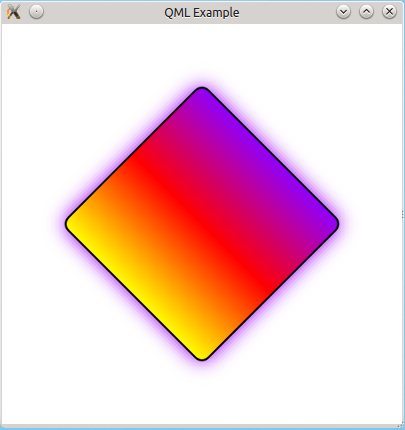
\includegraphics{img/qml.png}
\caption{Przykład wykorzystania QML}\label{rys:qml}
\end{figure}

\subsection{Własne elementy}
Istnieje możliwość tworzenia własnych elementów składających się z~elementów już dostępnych w~QML. Jednak bardzo złożone elementy, np. wykresy, łatwiej jest stworzyć w~C++, a następnie wyeksponować w~QML. Możliwe jest eksponowanie pojedynczych obiektów, jak i~eksportowanie całych klas. Aby klasa była zdatna do wykorzystania w~QML musi dziedziczyć po \textit{QObject}. Wyeksportowanie klasy odbywa się poprzez wywołanie jednej globalnej funkcji dostarczanej przez Qt. W~ten sposób zintegrowano z~QML chociażby bibliotekę Box2D.

\section{Założenia, cele i cechy biblioteki}
Podstawowym problemem bibliotek już dostępnych na rynku jest wąski zakres zastosowań. Dostarczane przez nie wykresy są zazwyczaj widgetami gotowymi do osadzenia w~GUI. Dla typowych aplikacji napisanych w~C++ może to być rozwiązanie wygodne, jednak ogranicza ono możliwości wykorzystania w~innym kontekście. Osadzenie widgetu w~dokumencie tekstowym lub w~\textit{GraphicsView} jest co najmniej nieefektywne. Stąd pierwszy z~celów stawianych mojej bibliotece -- dostarczenie uniwersalnego silnika, umożliwiającego wyświetlanie wykresów w~dowolnym miejscu aplikacji napisanych w~Qt. Na etapie definiowania wymagań ograniczyłem zbiór widoków, z~którymi moja biblioteka ma być kompatybilna, jednak teoretycznie powinna współpracować z~dowolnym widokiem.

Jak już wspomniałem we wstępie, Qt~Quick jest stosunkowo nową technologią i~cierpi na typowe schorzenie wieku dziecięcego -- ogarniczony zbiór bibliotek. Aktualnie na rynku istnieje tylko jedna biblioteka wspierająca tworzenie wykresów w~QML i~jest to rozwiązanie komercyjne. Istnieje duże zapotrzebowanie na wartościowe, darmowe rozwiązanie.

Celem Qt~Quick jest tworzenie intuicyjnych i~płynnie działających interfejsów użytkownika. Wykresy tworzone za pomocą mojej biblioteki wpisują się w~tę politykę. Istnieje możliwość animacji wielu właściwości elementów składowych wykresów. Same wykresy są również nastawione na interaktywne operacje, których zbiór jest co prawda ograniczony, jednak łatwy do rozszerzenia za pomocą systemu zdarzeń Qt.

Niektóre z~wymagań, głównie dostępność elementów wykresu z~poziomu QML, wymusiły na mnie specyficzną architekurę tej biblioteki. Intensywne wykorzystywanie mechanizmów dostarczanych przez \textit{QObject} oraz oszczędne korzystanie z~szablonów wpłynęły negatywnie na wydajność rozwiązania. Nie jest to jednak problem, gdyż podstawowym założeniem tego projektu było dostarczenie wykresów biurowych, które ze swej natury mają raczej statyczne źródła danych. Stąd też nazwa biblioteki -- \textit{Qt Office Charts}, która jednoznacznie sugeruje jej przeznaczenie. 

















\chapter{Przegląd dziedziny}
Rozdział ten zawiera opis kilku wybranych bibliotek służących do tworzenia wykresów. Opisałem tu  biblioteki przeznaczone dla Qt i~C++, podzielone na rozwiązania komercyjne oraz darmowe. Dla każdej biblioteki podałem jej zalety i~wady. Następnie przedstawiam wykaz typów wykresów dostępnych we wszystkich opisanych produktach. Kolejne dwa paragrafy to zestawienie elementów wspólnych i~unikalnych. Ostatni fragment to podsumowanie zawierające wnioski płynące z~tego przeglądu.

\section{Rozwiązania komercyjne}
\subsection{Qt Commercial Charts}
Biblioteka ta została stworzona przez aktualnego właściciela Qt, czyli firmę Digia. Oferuje ona programiście szeroki wybór wykresów. Nie wymaga zagłębiania się w~swoją wewnętrzną budowę, a~tworzenie prostych wykresów polega na połączeniu kilku wysokopoziomowych obiektów takich jak seria czy widget widoku.\newline

Cała biblioteka opiera się na frameworku Graphics View, który wprowadza podział na scenę oraz widok, gdzie scena jest kontenerem na elementy prezentowane za pomocą widoku.
Biblioteka udostępnia dwa uniwersalne widoki. Zależnie od zastosowania można użyć obiektu klasy dziedziczącej z~QGraphicsView bądź z~QGraphicsWidget. Implementacje konkretnych wykresów zarządzają elementami dodawanymi do sceny.\newline

Biblioteka ta, jako jedyna z tutaj opisanych, udostępnia wszystkie swoje wykresy w~języku QML, zarówno dla QtQuick~1~i~2.
Jak sam producent zaznacza, silne uzależnienie biblioteki od GraphicsView sprawia, że osiąga ona lepsze wyniki wydajnościowe dla QtQuick~1.\newline

\textbf{Zalety:}
\begin{itemize}
\item{szeroki wybór wykresów,}
\item{operowanie na komponentach wysokiego poziomu,}
\item{interaktywność wszystkich elementów wykresu,}
\item{system motywów umożliwiający tworzenie wykresów o~spójnej kolorystyce,}
\item{obiekty mapujące dane ze standardowych modeli Qt do serii danych,}
\item{wtyczka do Designera,}
\item{silne wsparcie dla QML.}\newline
\end{itemize}

\textbf{Wady:}
\begin{itemize}
\item{spadek uniwersalności poprzez uzależnienie prezentacji wykresów od konkretnych widoków,}
\item{wykorzystanie GraphicsView zamiast SceneGraph, powodujące niższą wydajność w QtQuick~2.}
\end{itemize}


\subsection{KD Charts}
Jest to biblioteka stworzona przez firmę KDAB~\footnote{KDAB \url{http://kdab.com}}. KD Charts w~odróżnieniu od poprzedniej biblioteki nie korzysta z~GraphicsView, a~z~mechanizmów niższego poziomu. Rysowanie odbywa się tu za pomocą systemu Arthur, a~do pisania wykorzystano silnik Scribe.
Dzięki wykorzystaniu technologii niższego poziomu, programistom KDAB udało się uzyskać lepszą wydajność, szczególnie ważną przy oferowanych przez nich wykresach czasu rzeczywistego.\newline

KD Charts separuje dane od warstwy prezentacji wykorzystując modele znane z~popularnego w~Qt wzorca Model-Widok. Za prezentację danych odpowiada uniwersalna klasa dziedzicząca po QWidget.\newline

\textbf{Zalety:}
\begin{itemize}
\item{szeroki wybór wykresów,}
\item{zbiór wbudowanych interakcji oraz możliwość tworzenia własnych,}
\item{duże możliwości parametryzowania wyglądu wykresu,}
\item{wykresy 2,5D,}
\item{wysoka wydajność, umożliwiająca tworzenie wykresów czasu rzeczywistego.}\newline
\end{itemize}

\textbf{Wady:}
\begin{itemize}
\item{wysoka cena,}
\item{wymuszenie korzystania z~modeli albo niskopoziomowych kontenerów do przechowywanie danych,}
\item{biblioteka napisana w~stylu Qt4, trudnym do wykorzystania w~QtQuick~2,}
\item{brak wsparcia dla QML.}
\end{itemize}

\subsection{QtitanChart}
Jest to biblioteka stworzona przez firmę Developer Machines, udostępniająca dosyć duży zbiór wykresów. Twórcy biblioteki nie udostępniają pełnych źródeł swojej biblioteki, a~jedynie jej pliki nagłówkowe i~biblioteki dynamiczne, co znacznie utrudnia zrozumienie jej wewnętrznego działania. Ta wiedza nie jest jednak potrzebna, gdyż aby tworzyć za jej pomocą wykresy, można się posługiwać komponentami wysokiego poziomu.\newline

\textbf{Zalety:}
\begin{itemize}
\item{szeroki wybór wykresów,}
\item{możliwość wyeksportowania wykresu do pliku graficznego,}
\item{możliwość wyświetlania wykresów różnych typów w~jednym układzie współrzędnych,}
\item{system motywów, umożliwiający tworzenie wykresów o~jednolitej kolorystyce.}\newline
\end{itemize}

\textbf{Wady:}
\begin{itemize}
\item{wysoka cena,}
\item{brak wsparcia dla QML.}
\end{itemize}


\section{Rozwiązania darmowe} 
\subsection{Qwt}
Qt Widgets for Technical Applications to otwarta biblioteka umożliwiająca tworzenie wykresów oraz innych widgetów technicznych. Biblioteka ta była projektowana z~myślą o zastosowaniach technicznych, w~szczególności w~systemach czasu rzeczywistego, przez co głównym celem było zapewne osiągnięcie wysokiej wydajności przy dynamicznie zmieniających się danych. Cel ten osiągnięto między innymi poprzez wykorzystywanie stosunkowo niskopoziomowych mechanizmów, jak Arthur czy intensywne wykorzystanie szablonów języka C++. Niestety przez to biblioteka nie jest szczególnie przyjazna użytkownikowi. Programista często musi sięgać do niskopoziomowych narzędzia, a stworzenie mniej standardowego rozwiązania może sprawić wiele trudności.\newline

Qwt zawiera szerokie API służące do przeprowadzania różnorakich operacji na wykresach, m.in. skalowania i zaznaczania. Problematyczną kwestią jest wygląd wykresów, z~jednej strony są one adekwatne dla zastosowań technicznych, z~drugiej zaś sprawia on, że nie sposób użyć tych wykresów w~aplikacji innego typu, ze względu na ich brzydotę. Najlepszym przykładem niech będzie wykres załączony na rys. \ref{rys:wykres:sinus}, wyglądający niczym oscylogram.
\begin{figure}
\centering
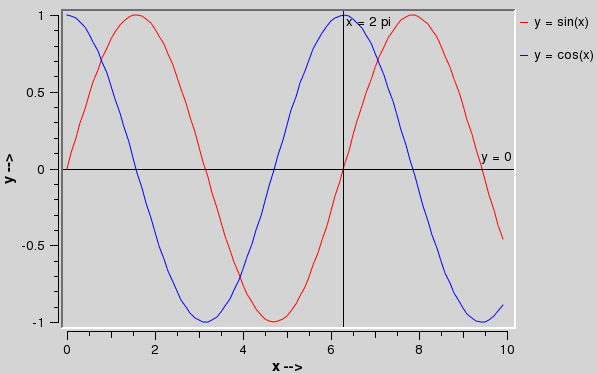
\includegraphics[scale=0.4]{img/sinus.png}
\caption{Przykładowy wykres Qwt}\label{rys:wykres:sinus}
\end{figure}

\textbf{Zalety:}
\begin{itemize}
\item{rozbudowane API,}
\item{wsparcie społeczności,}
\item{wysoka wydajność,}
\item{osie ze skalą logarytmiczną.}\newline
\end{itemize}

\textbf{Wady:}
\begin{itemize}
\item{nieprzyjazna użytkownikowi,}
\item{mało atrakcyjny wygląd wykresów,}
\item{brak wsparcia dla QML.}
\end{itemize}

\subsection{GobChartWidget}
Jest to jednoosobowy projekt rozwijany przez Williama Hallatta, dostępny na licencji open-source. Biblioteka ta ma bardzo ograniczoną funkcjonalność, pozwala na tworzenie wykresów tylko trzech typów: słupkowych, liniowych oraz kołowych, wszystkie o~bardzo prostym wyglądzie.\newline

Jest to kolejna biblioteka uzależniona od frameworku Model-Widok. Jest to jednak przypadek ekstremalny, nie polegający jedynie na trzymaniu danych w~modelu. Klasy odpowiedzialne za prezentację wykresów dziedziczą tu po abstrakcyjnym widoku z~ww. frameworku. Zapewne twórca uzyskał dzięki temu pewne ciekawe własności, jednak zmusiło go to do implementacji osobnych widoków dla każdego typu wykresu.\newline

Do rysowania wykresów wykorzystano tu GraphicsView, przy czym kontenerem na elementy nie jest scena, a~model.\newline

Jak widać GobChartWidget jest nieco dziwną hybrydą, której z~pewnością nie można nazwać skalowalną. Wcale nie dziwi fakt, że nie cieszy się ona szczególną popularnością wśród programistów Qt. Według statystyk SourceForge~\footnote{SourceForge \url{http://sourceforge.net}}, w~ciągu pół roku pobrano tę bibliotekę zaledwie kilkanaście razy.

\textbf{Zalety:}
\begin{itemize}
\item{darmowa,}
\item{najpopularniejsze wykresy,}
\item{współpraca z systemem Model-Widok}\newline
\end{itemize}

\textbf{Wady:}
\begin{itemize}
\item{ubogi zbiór wykresów,}
\item{mało przejrzysta struktura,}
\item{brak wspierającej społeczności programistów,}
\item{brak wsparcia dla QML.}
\end{itemize}



\section{Dostępne typy wykresów}
Podstawowym kryterium oceny użyteczności tego typu biblioteki jest zbiór wykresów, które udostępnia. Tablica~\ref{tab:wykresy} prezentuje dostępność typów wykresów w~opisanych bibliotekach.
\begin{table}[h]\footnotesize
\centering
\caption{Zestawienie dostępnych wykresów}
\label{tab:wykresy}
\begin{tabular}{|c|c|c|c|c|c|}
\hline
&  Qt Charts & KD Chart & Qtitan & Qwt & GobChart\\
\hline
Bąbelkowy & T & N & T & N & N\\
\hline
Gantta & N & T & N & N & N\\
\hline
Kołowy & T & T & T & N & T\\
\hline
Liniowy & T & T & T & T & T\\
\hline
Pierścieniowy & T & T & T & N & N\\
\hline
Słupkowy & T & T & T & N & T\\
\hline
Świecowy & T & T & N & N & N\\
\hline
Warstwowy & T & T & T & N & N\\
\hline
XY (punktowy) & T & N & T & T & N\\
\hline
\end{tabular}
\end{table}


\section{Elementy wspólne}
Analizując powyższe biblioteki dochodzę do wniosku, że można wykroić z nich część wspólną, stanowiącą podstawową funkcjonalność niezbędną dla biblioteki tego typu. Te elementy to:
\begin{itemize}
\item{podstawowe wykresy, takie jak liniowy, słupkowy i kołowy,}
\item{osie, siatka i legenda,}
\item{możliwość realizacji przez programistę interakcji z~użytkownikiem,}
\item{zaznaczanie i przybliżanie fragmentów wykresu,}
\item{serie danych -- każda z bibliotek wykorzystuje ujednolicony interfejs do danych. Czesem seria jest jedynie opakowaniem na kontener z~próbkami, innym razem zawiera większość logiki związanej z~konstrukcją wykresu,}
\item{efekty 2,5-3D, komercyjne biblioteki umożliwiają tworzenie pseudo-przestrzennych wykresów.}
\end{itemize}

\section{Elementy unikalne}
Prawie wszystkie biblioteki zawierają wartościowe elementy niepowtarzalne lub rzadko spotykane:
\begin{itemize}
\item{animacja towarzysząca tworzeniu wykresów oraz ich przebudowywaniu,}
\item{motywy pozwalające na tworzenie wykresów w~różnych, jednolitych stylach,}
\item{możliwość realizacji pełnej interakcji ze wszystkimi elementami wykresu,}
\item{możliwość konfiguracji elementu prezentującego kolor w~legendzie (np. koło dla wykresu bąbelkowego, odcinek dla liniowego),}
\item{generowanie plików graficznych zawierających wykresy,}
\item{możliwość wyświetlania kilku wykresów różnego typu w~jednym układzie współrzędnych,}
\item{nieliniowe skale osi,}
\item{wyeksponowanie klas C++ w QML.}
\end{itemize}

\section{Podsumowanie}
Na rynku istnieją już wartościowe biblioteki pozwalające na tworzenie wykresów biurowych, są to jednak rozwiązania komercyjne. Projekty open-source są albo niskiej jakości albo nadają się do innych (technicznych) zastosowań. Istnieje więc potrzeba stworzenia wysokiej jakości darmowego produktu, który zyskałby taką popularność jak Qwt. Potrzeba ta jest jeszcze większa dla Qt~Quick, gdzie nie ma żadnych darmowych bibliotek pozwalających na tworzenie wykresów.

Warto również zauważyć, że twórcy żadnej z~opisanych bibliotek nie zdecydowali się na pełne odizolowanie silnika biblioteki od widoków. Dzięki takiemu podejściu osiągnąłem możliwość wyświetlania wykresów w dowolnym miejscu -- wewnątrz widgetu, w~aplikacji napisanej w~QML czy w~dokumencie tekstowym. Jest to pierwsze takie rozwiązanie na rynku.



\chapter{Opis wymagań}
Istotą tego rozdziału jest opisanie wszystkich wymagań stawianych tworzonej bibliotece. 
Rozdział ten składa się z~dwóch głównych części: opisu wymagań funkcjonalnych i~opisu wymagań pozafunkcjonalnych.

Opis wymagań funkcjonalnych rozpoczynają wymagania stawiane całej bibliotece oraz wymagania odnoszące się do wszystkich tworzonych za jej pomocą wykresów. Następnie zostały przedstawione specyficzne wymagania dotyczące konkretnych typów wykresów.

Opis wymagań pozafunkcjonalnych został dokonany w~kontekście całej biblioteki, a~w~jego skład wchodzą rozważania na temat takich zagadnień jak skalowalność, wydajność czy niezawodność.

%\section{Wspólne wymagania funkcjonalne}

\section{Wykresy biurowe}
Za pomocą projektowanej biblioteki programiści będą mieć możliwość tworzenia interaktywnych wykresów typu biurowego. Po lekturze rozdziału poświęconego przeglądowi dziedziny wiadomo już, że zbiór wykresów biurowych jest dość liczny. Z~drugiej strony łatwo zauważyć, że jeden podzbiór wykresów jest szczególnie popularny. Projektując tę bibliotekę staram się skupić na stworzeniu elastycznej architektury, a~nie na udostępnieniu jak największej liczby typów wykresów. W~pierwszej wersji biblioteki zbiór wykresów będzie dośc ubogi i~będzie zawierał jedynie te najpopularniejsze.

\subsection{Dostępne wykresy}
Biblioteka musi udostępniać następujące typy wykresów:
\begin{itemize}
\item{kołowy}
\item{słupkowy}
\item{liniowy}
\end{itemize}

%Specyficzne wymagania dotyczące wykresów każdego z~tych typów zostały podane w~dalszej części rozdziału.

\subsection{Inne wykresy}
Architektura biblioteki musi umożliwiać dodawanie nowych typów wykresów biurowych. Mechanizmy takie jak współpraca ze źródłami danych lub podłączenie widoku do wykresu powinny być na tyle uniwersalne, aby nie wymagały jakichkolwiek modyfikacji dla wykresów nowych typów. W~idealnym scenariuszu stworzenie nowego wykresu powinno ograniczyć się do zaimplementowania jego wewnętrznej logiki oraz wykorzystania już istniejących komponentów, np. legendy, bez ich modyfikacji.
 
\section{Uniwersalny silnik}
Podstawowym celem projektowanej biblioteki jest udostępnienie programistom uniwersalnego silnika umożliwiającego tworzenie interaktywnych wykresów. Ma to być rozwiązanie generyczne, działające zarówno dla klasycznego Qt jak i~Qt~Quick~2. Tworzony silnik powinien umożliwiać wyświetlenie wykresów w~następujących miejscach:
\begin{itemize}
\item{widgety,}
\item{architektura Graphics View,}
\item{dokumenty tekstowe,}
\item{QML.}
\end{itemize}

W~tablicy~\ref{tab:widoki} zostały podane stosowne dla każdego z~przypadków wykorzystania widoki.

\begin{table}[h]\footnotesize
\centering
\caption{Widoki kompatybilne z~moją biblioteką}
\label{tab:widoki}
\begin{tabular}{|c|c|}
\hline
Miejsce & Klasa bazowa widoku\\
\hline
Widget & QWidget\\
\hline
Graphics View & QGraphicsObject\\
\hline
Dokument tekstowy & QTextFrame\\
\hline
QML & QQuickItem -- klasy bazujące na SceneGraph\\
 & QQuickPaintedItem -- klasy bazujące na QPainter\\
\hline
\end{tabular}
\end{table}


\section{Źródła danych}
Typowym źródłem danych jest seria, czyli swego rodzaju pojemnik na próbki. Każde źródło danych, którym ma być zasilany wykres, musi udostępniać zbiór danych o~następującej strukturze:

\begin{itemize}
\item{jedna liczba ze specyficznego dla danego przypadku zbioru wartości, będącego podzbiorem zbioru liczb rzeczywistych}
\item{co najmniej jedna wartość z~dziedziny liczb rzeczywistych. Bardziej złożone wykresy mogą mieć kilka takich wartości.}
\item{tytuł próbki}
\item{kolor}
\end{itemize}

Zakładam, że serie zawierają maksymalnie jedną próbkę dla danego wektora z~dziedziny. 

Ponadto wymagany jest tytuł i~kolor dla każdej z~serii.


\subsection{Serie danych}
Istnieje potrzeba stworzenia prostego i~lekkiego modelu danych reprezentującego serie, które z~kolei zawierają próbki. Niezbędne są operacje dodawania, modyfikowania i~usuwania danych z~serii. 

Aby ułatwić programistom Qt zapoznanie się ze sposobem działania mojej biblioteki, powinienem skorzystać tutaj ze statycznego polimorfizmu. Interfejs serii danych powinien przypominać interfejs modelu z~architektury Model-Widok.

\subsection{Model--Widok}
Wykresy mają być alternatywą dla widoków z~architektury Model-Widok. Uważam, że typowym przypadkiem użycia będzie prezentowanie tych samych danych za pomocą wykresów oraz tabelek. Z~tego powodu wszystkie wykresy muszą przyjmować jako źródło danych obiekty klas dziedziczących po \textit{QAbstractItemModel}.

%\subsection{Modele w QML}
%Szczególnymi przypadkami modeli są te wykorzystywane w~QML. Ważne jest, aby podłączenie elementów \textit{ListModel}~\footnote{ListModel \url{http://qt-project.org/doc/qt-5.1/qtqml/qml-qtqml-models2-listmodel.html}} i~\textit{XmlListModel}~\footnote{XmlListModel \url{http://qt-project.org/doc/qt-5.0/qtquick/qml-qtquick-xmllistmodel2-xmllistmodel.html}} do wykresu było intuicyjne dla programistów QML i~ograniczało się do jednej operacji:
%\begin{lstlisting}
%model: xmlModel
%\end{lstlisting}

\section{Interaktywność}
Celem tej pracy jest stworzenie biblioteki ,,do operowania na wykresach''. Wszystkie wykresy muszą obsługiwać interaktywne operacje, a~część z~nich powinna zostać zaimplementowana. Pozostałe powinny być możliwe do realizacji.

\subsection{Zaznaczanie}
Musi istnieć możliwość zaznaczania elementów reprezentujących dane. Powinna istnieć możliwość zaznaczania zarówno elementów reprezentujących pojedyncze próbki, np. wycinek kołowy, jak i~tych tych odpowiadających całym seriom danych, np. grupa słupków. Zaznaczanie powinno być możliwe poprzez kliknięcie przyciskiem myszy lub dotknięcie ekranu dotykowego.

\subsection{Modyfikacja zawartości modelu}
Powinna istnieć możliwość zmiany zawartości modelu poprzez interakcję z~wykresem. Dla danego elementu reprezentującego próbkę, zmiana jego parametru proporcjonalnego do reprezentowanej wartości powinna skutkować zmianą danych zawartych w~modelu. I~tak skrócenie słupka powinno spowodować zmniejszenie odpowiedniej wartości w~modelu, a~zwięszkenie kąta rozwarcia wycinka kołowego zwiększenie analogicznej wartości.

\subsection{Inne operacje}
Architektura biblioteki powinna umożliwiać programistom realizację innych interaktywnych operacji, np. system \textit{Przeciągnij i~Upuść}. Powinno być to możliwe poprzez wykorzystanie systemu zdarzeń Qt.

%\subsection{API w stylu Qt}


\section{Qt~Quick}
Projektując tę bibliotekę muszę wziąć pod uwagę jej późniejsze zastosowanie, którym ma być m.in. tworzenie wykresów w~QML. 

\subsection{Wyeksponowanie klas C++ w QML}
Już na etapie projektowania należy zadbać, aby tworzone struktury były łatwe do wyeksponowania w~QML. 
Tworzenie interfejsów do QML nie jest celem tego projektu, jednak ich implementacja powinna być możliwie łatwa dla programistów decydujących się na korzystanie z~mojej biblioteki.

\subsection{Delegaty}
Szeroko stosowanym w~Qt~Quick mechanizmem są delegaty. Umożliwiają one zdefiniowanie przez programistę sposobu prezentacji danych z~modelu. W~mojej bibliotece korzystanie z~delegatów powinno być możliwe w~legendzie, do prezentacji kolorów, oraz we właściwym wykresie do definiowania własnych elementów prezentujących zawartość modelu, np. słupki.


\section{Wspólne elementy składowe}
Wszystkie wykresy muszą zawierać następujące elementy:
\begin{itemize}
\item{źródło danych,}
\item{elementy prezentujące pojedyncze próbki danych (słupek, punkt, wycinek kołowy),}
\item{tytuł wykresu,}
\item{legenda,}
\item{dodatkowe elementy dostarczane przez programistów.}
\end{itemize}

Wyświetalnie każdego z~elementów wykresu powinno być sterowane przez programistę. Powinna również istnieć możliwość ustawienia tła wykresu.

 
\subsection{Elementy prezentujące dane}
Każdy z~wykresów posiada specyficzny dla niego element służący do prezentacji danych z~próbki, którego rozmiar lub położenie w~układzie współrzędnych odzwierciedla wartość próbki. Każdy z~elementów może mieć swój podpis. Powinna istnieć możliwość ustawienia tym elementom dwóch piór i~dwóch pędzli -- dla trybu normalnego i~zaznaczenia. Programista powinien mieć możliwość podmiany, dla danego wykresu, klasy takiego elementu na własną, przy czym odpowiedzialność za poprawne odrysowanie się wykresu spada wtedy na programistę.

\subsection{Tytuł wykresu i podpisy elementów}
Dla wszelkich napisów będących składowymi wykresu musi być możliwość ustawienia ich treści, czcionki oraz koloru.

\subsection{Legenda}
Dla wykresów obsługujących wiele serii danych legenda powinna prezentować kolory oraz tytuły tych serii. Natomiast dla wykresów jednoseryjnych prezentowana powinna być informacja o~kolorze i~tytule każdej z~próbek. Legenda powinna przyjmować jedno z~dwóch położeń -- poziome lub pionowe. Powinna istnieć możliwość zmiany elementu prezentującego kolor za pomocą mechanizmu delegatów.

\subsection{Dodatkowe elementy}
Programiści powinni mieć możliwość tworzenia własnych elementów i~dodawania ich do wykresów już istniejących klas. Aby to osiągnąć powinni jedynie zaimplementować odpowiednie interfejsy.


%\section{Dostępne operacje na wykresach}
\section{Skalowanie}
Powinno być możliwe skalowanie wykresu. Wykres powinien dostosowywać swój rozmiar do przekazanego mu obszaru przeznaczonego na jego odrysowanie.



\section{Wykresy w układzie współrzędnych}
Niektóre wykresy wymagają osadzenia w~układzie współrzędnych. Takie wykresy wymagają dodatkowych elementów:

\begin{itemize}
\item{osie}
\item{siatka}
\end{itemize}

\subsection{Osie}
Powinna istnieć możliwość przypisania do osi skali innej niż liniowa.
Powinna być możliwość ustawienia pióra służącego do rysowania osi, jej tytułu, gęstości ticków oraz zakresu wartości. 

\subsection{Siatka}
Powinna istnieć możliwość określenia grubości i~koloru linii oraz ziarnistości samej siatki.

\subsection{Układy współrzędnych}
Mimo iż dziedzinie wykresów najpopularniejszym układem współrzędnych jest układ kartezjański, w~projekcie należy uwzględnić istnienie innych układów współrzędnych takich jak biegunowy czy cylindryczny.

\subsection{Wspólny układ współrzędnych}
Powinna istnieć możliwość wyświetlania kilku wykresów, również różnych typów, w~jednym układzie współrzędnych.





\section{Wykres kołowy}
Wykres kołowy służy do prezentacji danych z~jednej serii. Każda z~próbek jest prezentowana za pomocą wycinka kołowego o~kącie środkowym proporcjonalnym do prezentowanej wartości, przez co muszą to być wartości rzeczywiste dodatnie. Wartości wszystkich próbek serii sumują się do stu procent, a~suma kątów wewnętrznych wycinków wynosi 360 stopni. Wszystkie wycinki z~danej serii mają wspólny środek oraz jednakowy promień.

\subsection{Przemieszczanie wycinka}
Dowolny z~wycinków powinno się dać przesunąć o~zadaną część jego promienia. Proces ten powinien być możliwy do animacji z~zastosowaniem standardowych rozwiązań Qt.

\subsection{Obracanie wykresu}
Powinna być możliwość obracania wykresu wokół jego środka. Kąt obrotu powinien być dowolną całkowitą wartością, o~jednostce wynoszącej $\dfrac{1}{16}$ stopnia -- jest to standardowa w~Qt jednostka. Proces ten powinien być możliwy do animacji.
 

\section{Wykres słupkowy}
Jest to wykres służący do prezentacji danych z~wielu serii. Elementem odpowiedzialnym za prezentację pojednyczej próbki jest tu słupek. Wszystkie słupki danej serii mają ten sam kolor. W~ogólnym przypadku za pomocą tego wykresu można prezentować wartości z~dziedziny liczb rzeczywistych.

\subsection{Układ słupków} 
Wykres słupkowy może przyjmować układ pionowy bądź poziomy. Wykres z~pionowym układem słupków jest  nazywany wykresem kolumnowym i~został przedstawiony na rysunku~\ref{rys:wykres:pion}. Natomiast przykładowy wykres z~poziomym układem znajduje się na rysunku~\ref{rys:wykres:poziom}.

\begin{figure}[H]
\centering
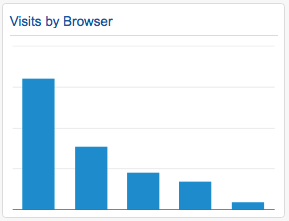
\includegraphics[scale=0.8]{img/bar-ver.png}
\caption{Pionowy układ słupków}\label{rys:wykres:pion}
\end{figure}

\begin{figure}[H]
\centering
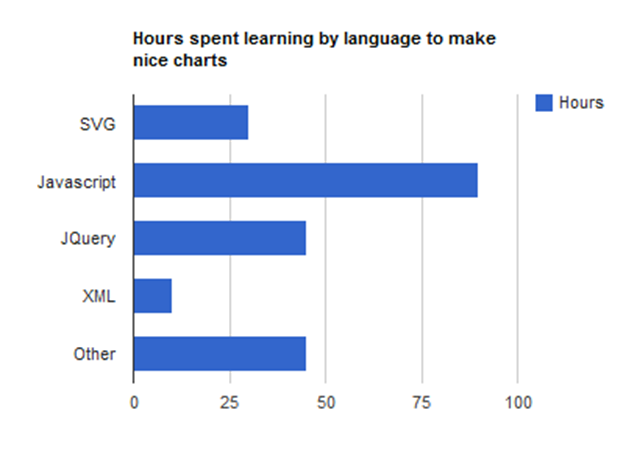
\includegraphics[scale=0.8]{img/bar-hor.png}
\caption{Poziomy układ słupków}\label{rys:wykres:poziom}
\end{figure}

\subsection{Stos}
Wykres słupkowy może zostać przedstawiony w~trybie stosowym. Wtedy dla każdej wartości z~dziedziny tworzony jest jeden słupek o~wysokości proporcjonalnej do sumy wartości próbek ze wszystkich serii wykresu. Z~kolei ten słupek jest podzielony na mniejsze cześci o~długościach i~kolorach odpowiednich próbek. Na rysunku~\ref{rys:wykres:stos} przedstawiam przykład stosowego wykresu słupkowego.

\begin{figure}[H]
\centering
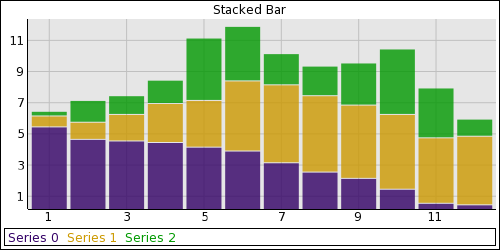
\includegraphics[scale=0.8]{img/stacked-bar.png}
\caption{Stosowy wykres słupkowy}\label{rys:wykres:stos}
\end{figure}


\section{Wykres liniowy}
W wykresie liniowym dana próbka jest prezentowana za pomocą pojedynczego punktu. Punkty są prezentowane jako koła o~zadanym promieniu. Wartości próbek należą do zbioru liczb rzeczywistych. Punkty danej serii mogą zostać połączone w~łamaną.

\subsection{Łączenie punktów}
Programista powinien mieć możliwość podjęcia wyboru w~kwestii łączenia punktów w~łamaną. Powinien mieć również możliwość zmiany wszystkich parametrów łamanej, tak jak dla elementów odpowiedzialnych za prezentację próbek.

\section{Dodatki}
Wszystkie opisane tu funkcjonalności są opcjonalne, a~ich realizacja nie jest konieczna do zakończenia prac nad biblioteką.

\subsection{Motywy}
Dodatkiem, który podniósłby atrakcyjność wykresów jest wysokopoziomowy mechanizm motywów, podobny do \textit{QStyle}. Mechanizm ten powinien umożliwiać tworzenie wykresów o~spójnej kolorystyce oraz czcionkach. Zmiana motywu dla danego wykresu powinna sprowadzać się do prostej operacji.

\subsection{Budowanie wykresu}
Powinno być możliwe animowanie procesu budowania wykresu. Podczas tego procesu kolejne elementy wykresu będą stawały się widoczne, a~elementy odpowiedzialne za prezentację danych powinny stopniowo przyjmować swoje wartości, począwszy od zera.

\subsection{Generowanie plików graficznych}
Powinno być możliwe generowanie na podstawie istniejących wykresów plików graficznych  w~formatach PNG i~SVG.

\section{Przenośność}
Biblioteka musi wpisywać się w~politykę Qt brzmiącą: \textit{pisz raz, kompiluj wielokrotnie}. Musi być przenośna na poziomie kodu źródłowego między najważniejszymi wspieranymi przez Qt platformami.
Minimum to uruchomienie na systemach:
\begin{itemize}
\item{Windows,}
\item{Linux.}
\end{itemize}


\section{Wymagania pozafunkcjonalne}
Wymagania funkcjonalne nie są jedynymi kryteriami oceny biblioteki. Równie ważne są wymagania definiujące oczekiwania użytkownika na temat budowy biblioteki oraz wynikające z~niej ograniczenia dotyczące wydajności czy skalowalności. Poniżej poruszam te i~kilka innych kwestii nie związanych bezpośrednio z~funkcjonalnością.

\subsection{API w stylu Qt}
%API tworzonej przeze mnie bilioteki powinno posiadać jak najwięcej z sześciu cech charakteryzujących %dobre interfejsy programistyczne:
%\begin{itemize}
%\item{minimalne,}
%\item{kompletne,}
%\item{intuicyjne,} 
%\item{łatwe do zapamiętania,}
%\item{czysta i~prosta semantyka,}
%\item{czytelny kod.}
%\end{itemize}

%Jednak nie są to wszystkie wymagania stawiane projektowanej bibliotece. 

Aby tworzony przeze mnie kod był czytelny dla innych programistów Qt, musi on wykorzystywać standardowe mechanizmy tej platformy:
\begin{itemize}
\item{statyczny polimorfizm, polegający na tworzeniu podobnych interfejsów dla podobnych, ale niespokrewnionych klas, np. kontenerów. Zastępuje wprowadzanie sztucznych klas bazowych.}
\item{właściwości jako sposób na parametryzowanie obiektów,}
\item{preferowanie przyjmowania wskaźników zamiast referencji do funkcji modyfikujących argumenty,}
\item{asynchroniczna komunikacja między obiektami rozwiązana za pomocą sygnałów i~slotów,}
\item{nazewnictwo, sposób zwracania wartości z~funkcji i~wiele innych opisanych w~\cite{APIDesign}.}
\end{itemize}

\subsection{Wymienność biblioteki}
Biblioteka powinna wykorzystywać mechanizmy pozwalające na tworzenie bibliotek dynamicznych wymiennych pomiędzy wersjami. Wprowadzenie nowej wersji biblioteki z~niezmienionym interfejsem nie powinno wymagać przebudowania całej aplikacji z~niej korzystającej.

\subsection{Nowoczesność i~uniwersalność}
Biblioteka powinna wykorzystywać możliwie nowe technologie, np. Qt5. Biblioteka może korzystać z~\textit{C++11}, jednak nie powinna wymuszać na użytkowniku posiadania kompilatora zgodnego z~tym standardem. Komponenty dostarczane do użytku programistom powinny być możliwie wysokopoziomowe i~uniwersalne w~użyciu.

\subsection{Wydajność}
Jako, że okoliczności wykorzystania wykresów biurowych są inne niż wykresów technicznych oraz natura ich danych jest dużo bardziej statyczna, optymalizacja nie jest tu kwestią najważniejszą. 
Z~tego powodu oraz z~chęci uniknięcia antywzorca projektowego przedwczesnej optymalizacji, kwestie wydajności bilioteki jest odsuwana na dalszy plan.

\subsection{Niezawodność}
Jak już wspomniałem w~poprzednim punkcie, natura oraz zastosowania wykresów biurowych różnią się od technicznych, a~co za tym idzie, mają również inne wymagania dotyczące niezawodności. Przewiduje się, że biblioteka będzie przeznaczona do aplikacji finansowych i~biurowych, a nie systemów czasu rzeczywistego. Jednakowoż w~celu minimalizacji liczby błędów w~kodzie, powinny zostać zastosowane testy regresji. Zachowanie biblioteki w warunkach ekstremalnych, np. ograniczonego dostępu do zasobów, nie jest głównym celem projektu.

%\subsubsection{Wiarygodnosć}

\subsection{Skalowalność}
Zarówno dodawanie nowych jak i~usuwanie już istniejących elementów biblioteki powinno być łatwe i~nie powinno mieć wpływu na stabilność pracy biblioteki. Dodawanie nowych elementów powinno być możliwe dzięki uniwersalnym interfejsom. Natomiast usuwanie istniejących elementów powinno sprowadzać się do wyłączenia ich z~procesu budowania biblioteki.

\chapter{Analiza wymagań}
Mimo iż poprzedni rozdział daje już dość klarowny obraz celu, do jakiego dążę przy projektowaniu tej biblioteki, w~niniejszym rozdziale dokonuję analizy niektórych z~wymagań. Rozpoczynam od diagramu poziomu zero~\ref{rys:use:cases}, który zawiera wszystkie najważniejsze wymagania wysokiego poziomu. Kolejne podrozdziały zawierają tekstowy opis scenariuszy. 

W~rozdziale tym starałem się nie nadużywać diagramów, gdyż ,,diagramy przypadków użycia i~związki pomiędzy przypadkami mają drugorzędne znaczenie w~procesie analizy wymagań. Przypadki użycia to dokumenty tekstowe. Tworzenie przypadków użycia sprowadza się do pisania tekstu''. Autorem tych słów jest Craig Larman, autor książki poświęconej projektowaniu oprogramowania~\cite{UML:Wzorce}.

\begin{figure}[H]
\centering
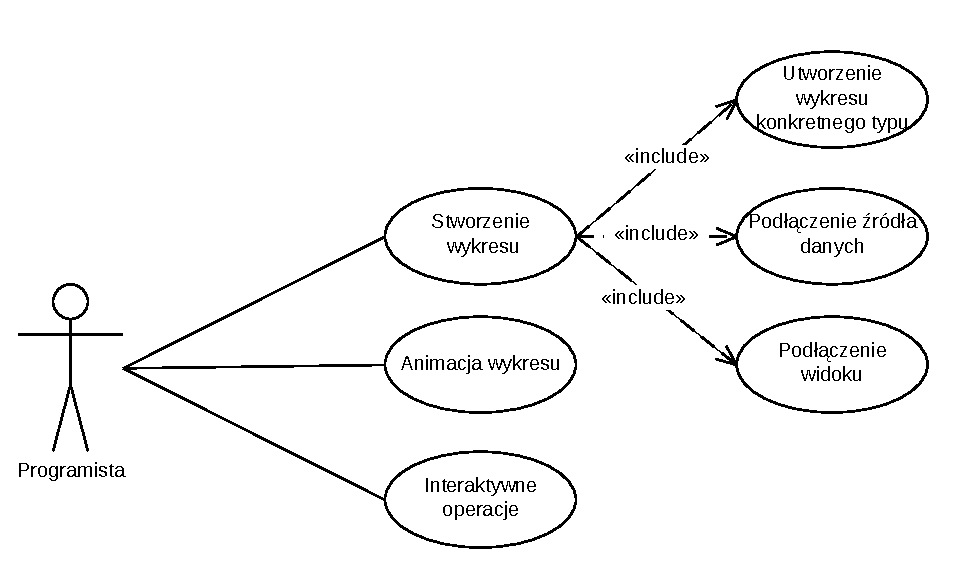
\includegraphics[scale=0.9]{img/use_case.pdf}
\caption{Diagram przypadków użycia poziomu zero}\label{rys:use:cases}
\end{figure}

\section{Stworzenie wykresu}
Stworzenie oraz wyświetlenie wykresu prezentującego dane z~określonego źródła składa się z~trzech głównych etapów, które postanowiłem opisać nieco bardziej szczegółowo.

\subsection{Utworzenie wykresu konkretnego typu}
\begin{enumerate}
\item{Programista wybiera typ wykresu i~tworzy obiekt tego typu.}
\item{Jeśli dany wykres istnieje w~kilku rodzajach, programista wybiera jeden z~nich. Wykres domyślnie przyjmuje określony rodzaj.}
\item{Programista ustawia wartości parametrów wykresu związanych z~jego odrysowywaniem, np. włączenie antyaliasingu.}
\item{Programista ustawia parametry wykresu charakterystyczne dla jego typu.}
\end{enumerate}

\subsection{Podłączenie źródła danych}
\begin{enumerate}
\item{Programista rejestruje wybrany przez siebie typ źródła danych jako \textit{QVariant}.}
\item{Programista tworzy źródło danych tego typu.}
\item{Programista wykorzystuje metodę wykresu do połączenia źródła danych z~wykresem.}
\item{Programista uzupełnia źródło danymi.}
\item{Wykres reaguje na zmianę danych poprzez ponowne odrysowanie.}
\end{enumerate}

\subsection{Podłączenie widoku}
\begin{enumerate}
\item{Programista wybiera widok, w~którym odrysowywany będzie wykres.}
\item{Programista tworzy klasę dziedziczącą po odpowiedniej klasie widoku, zgodnie z~tablicą~\ref{tab:widoki}.}
\item{Programista realizuje opisany w~rozdziale \textit{Projekt} protokół komunikacji pomiędzy widokiem a wykresem.}
\end{enumerate}


\section{Animacja wykresu}
Animacja elementów wykresu ma być możliwa poprzez wykorzystanie standardowych mechanizmów Qt.
\begin{enumerate}
\item{Programista wybiera element oraz jego właściwość, której wartość ma podlegać animacji.}
\item{Programista wybiera interesujący go typ animacji, ustawia jej parametry i~aktywuje na wybranej właściwości elementu wykresu.}
\item{Kolejne zmiany wartości właściwości powodują powiadomienie widoku wykresu o~potrzebie odrysowania.}
\item{Wykres jest odrysowywany z~uwzględnieniem zmian wynikających z~animacji.}
\end{enumerate}

\section{Interaktywne operacje}
Poniżej opisuję scenariusz potyczący dowolnej interaktywnej operacji możliwej do zaimplementowania w~ramach zaprojektowanej przeze mnie architektury.

\begin{enumerate}
\item{Programista odblokowuje daną interaktywną operację dla danej instancji wykresu.}
\item{Widok dostarcza przeznaczone dla wykresu zdarzenie.}
\item{Wykres decyduje, którego z~elementów dotyczy zdarzenie.}
\item{Wykres decyduje czy dane zdarzenie powoduje zmianę w~jego stanie, jeśli tak to podejmuje odpowiednią akcję.}
\item{Wykres powiadamia widok o potrzebie odrysowania.}
\item{Wykres jest odrysowywany z~uwzględnieniem zmian wynikających z~interakcji.}
\end{enumerate}









\chapter{Projekt}
Rozdział ten zawiera inżynierski projekt rozwiązań dla wymagań z~poprzednich rozdziałów. Poza opisem tekstowym, zastosowałem w~nim diagramy klas oraz sekwencji UML.

\section{Podział na warstwy}
Zdecydowałem się podzielić wykres na pięć warstw. Odrysowywanie wykresu będzie się składało z~odrysowania zawartości każdej z~warstw, począwsze od tła, a~na pierwszym planie skończywszy.
Układ warstw został przedstawiony na rysunku~\ref{rys:warstwy}.

\begin{figure}[H]
\centering
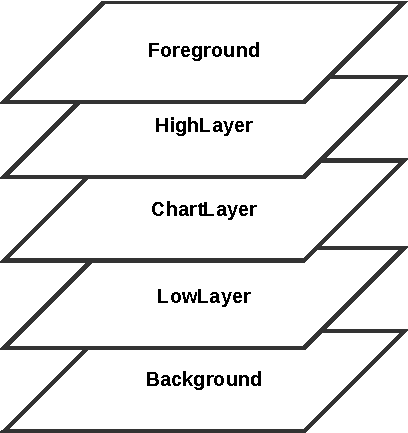
\includegraphics{img/warstwy.pdf}
\caption{Warstwy wykresu}\label{rys:warstwy}
\end{figure}

Warstwy tła oraz pierwszego planu służą jedynie odrysowywaniu wzorów przekazanych za pomocą pędzla. Pozostałe warstwy są bardziej złożone i~zawierają liczne elementy.

Warstwy niska i~wysoka są odrysowywane zgodnie z~algorytmem malarza. Służą dodawaniu przez programistów własnych elementów do wykresów istniejących klas.

Warstwa wykresu służy odrysowaniu głównej zawartości wykresu. Tym etapem steruje strategia danego wykresu. W~ogólnym przypadku programiści nie powinni dodawać własnych elementów do tej warstwy.

%\subsection{Metoda szablonowa}
Metoda odpowiedzialna za odrysowywanie wykresu powinna być \textit{Metodą Szablonową}~\cite{Patterns}, czyli niewirtualną, publiczną metodą klasy bazowej, wywołującą kolejne metody odpowiedzialne za odrysowanie pojedynczych warstw. Metody te powinny z~kolei być wirtualne i~chronione.
Metody odpowiedzialne za tło i~pierwszy plan powinny udostępniać domyślną implementację, natomiast pozostałe powinny być czysto wirtualne.

\section{Lokalny układ współrzędnych}
Każdy z~wykresów będzie posiadać lokalny, kartezjański układ współrzędnych rzeczywistych. Ponadto granice wykresu będą wyznaczane przez specjalny prostokąt. Takie podejście umożliwi układanie elementów względem lokalnego, a~nie globalnego układu współrzędnych, oraz ustalanie, które z~elementów są widoczne i~należy je odrysować. Dodatkowo ułatwiona będzie realizacja takich wymagań jak: skalowanie wykresu czy interaktywność. 

\begin{figure}[H]
\centering
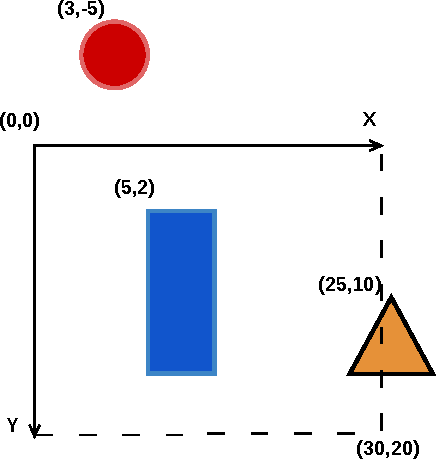
\includegraphics{img/uklad_wspolrzednych.pdf}
\caption{Lokalny układ współrzędnych}\label{rys:uklad:wspolrzednych}
\end{figure}

Na rysunku~\ref{rys:uklad:wspolrzednych} przedstawiono przykładowy układ współrzędnych wykresu o~wymiarach 30x20. W~tej sytuacji prostokąt zostanie wyświetlony w~całości, trójkąt tylko częściowo, a~koło wcale nie zostanie wyświetlone.


\section{Struktura wykresu}
Ogólna koncepcja na strukturę wykresu została przedstawiona na diagramie~\ref{rys:klasy:top_level}.

Klasy pochodne od QocAbstractChart są miejscem łączącym wszystkie inne elementy. To na nich będą ustawiane parametry odnoszące się do całości wykresu, np. włączenie antyaliasingu.

QocSeries odpowiada za dane dostarczane do wykresu. Jest lekkim odpowiednikiem modelu z~architektury Model-Widok.

QocAbstractStrategy to klasa bazowa dla strategii -- layoutu, odpowiedzialnego za odpowiednie układanie elementów wykresu, głównie z~warstwy środkowej -- \textit{ChartLayer}, i~ich odrysowywanie. Jest to szczególnie przydatny komponent dla wykresów, które mogą być budowane na różne sposoby, np. wykres słupkowy.


\begin{figure}[H]
\centering
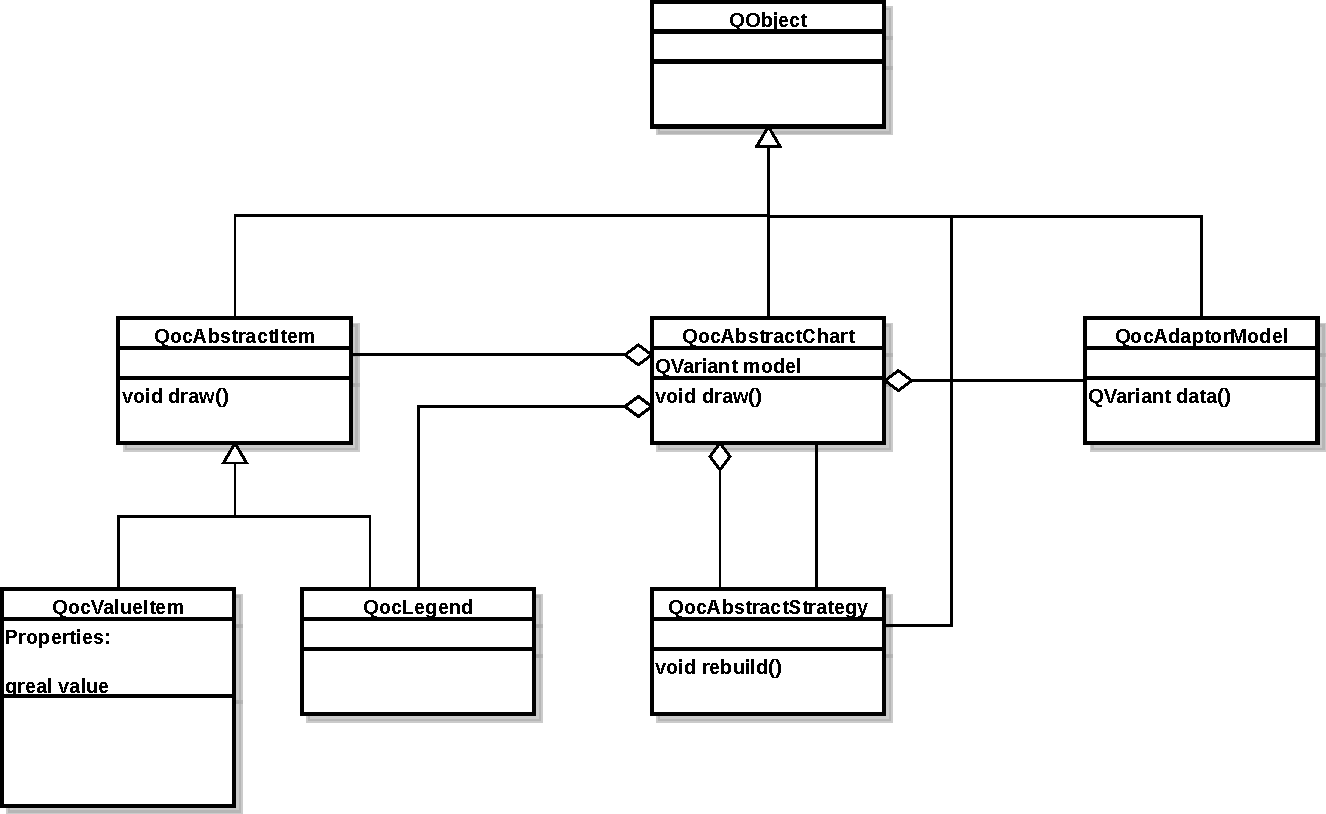
\includegraphics[scale=0.7]{img/klasy-top_level.pdf}
\caption{Diagram top level}\label{rys:klasy:top_level}
\end{figure}

\section{Źródła danych}

Jako że źródłem danych dla wykresu może być seria danych, zbiór serii albo model, postanowiłem wprowadzić pośrednią klasę, która będzie odpowiedzialna za unifikację komunikacji wykresu ze źródłem danych. Klasa ta będzie \textit{Adapterem obiektowym}~\cite{Patterns} -- będzie agregowała źródła danych dostarczane jako obiekty \textit{QVariant}. Hierarchię klas związanych z~adapterem przedstawiłem na diagramie~\ref{rys:adapter:model}

\begin{figure}[H]
\centering
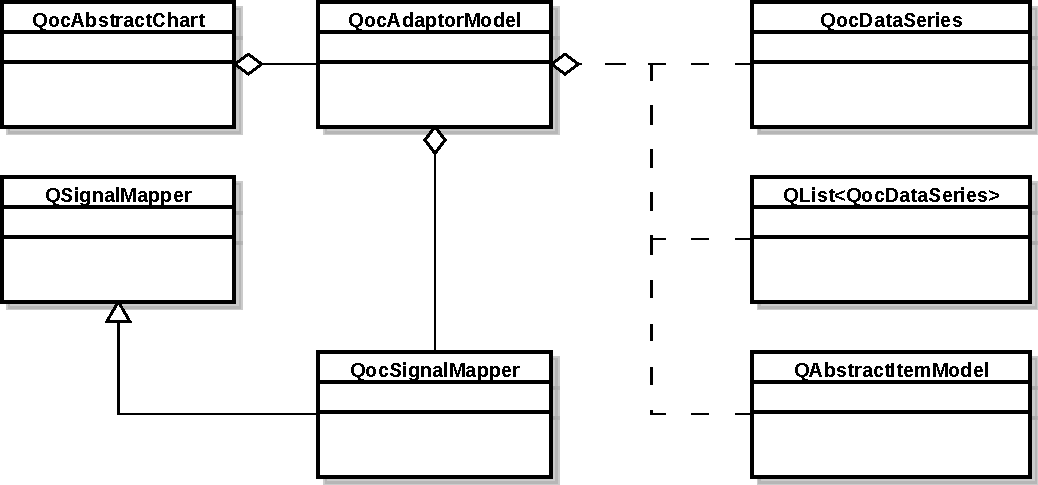
\includegraphics[scale=0.8]{img/adapter-model.pdf}
\caption{Adapter}\label{rys:adapter:model}
\end{figure}

Za pomocą adaptera stworzę pewną abstrakcję, dzięki której niezależnie od klasy źródła danych, wykres zawsze będzie go postrzegał jako zbiór serii. Większość metod adaptera, jako jeden z~argmuentów będzie przyjmować identyfikator serii, dzięki czemu będzie można wyspecyfikować  której serii dotyczy dana operacja. 

Komunikacja w~drugą stronę zostanie rozwiązana za pomocą zbioru sygnałów, które również będą niosły informację o~id serii. W~przypadku zbioru serii, wystarczy uzupełnić ich sygnały o~id serii oraz przepropagować na zewnątrz adaptera. Chcę to osiągnąć za pomocą obiektu klasy pochodnej od \textit{QSignalMapper}~\footnote{QSignalMapper \url{http://qt-project.org/doc/qt-5.0/qtcore/qsignalmapper.html}}. W~przypadku klas modeli, również będę musiał wykonać podobne mapowanie, podczas którego trzeba będzie sięgnąć do modelu po id serii. Przykładowy protokół komunikacji wykresu z~adapterem przedstawiłem na rysunku~\ref{rys:wykres:model}.

\begin{figure}[H]
\centering
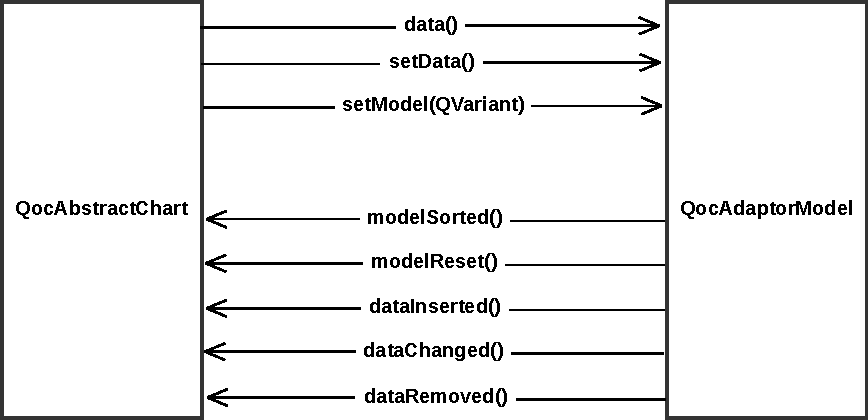
\includegraphics[scale=0.8]{img/wykres-model.pdf}
\caption{Komunikacja Wykres -- Adapter}\label{rys:wykres:model}
\end{figure}

\subsection{Role}
Wzorując się na systemie Model-Widok, zdecydowałem się wprowadzić do mojej biblioteki byt o~nazwie: Rola. Rola to typ wyliczeniowy, który służy do wskazania przez widok, jakich danych oczekuje od modelu. Widok chcąc uzyskać dane z~modelu musi mu przekazać indeks i~właśnie rolę.

Dzięki rolom uzyskam stan, w~którym wykres chcąc pobrać dane z~modelu, przekaże do adaptera rolę. Adapter zajmie się przetłumaczeniem roli. W~zależności od kontekstu, może to być numer kolumny, rola  albo właściwość obiektu.

\begin{lstlisting}[caption=Rola -- typ wyliczeniowy, label=code:role]
enum Role{
	XRole,
	YRole,
	TitleRole,
	ColorRole,
	CustomRole
}
\end{lstlisting}

%Każda z~wartości tego~\ref{code:role} typu wyliczeniowego musi posiadać odpowiadający jej łańcuch znaków. Dwukierunkowe mapowanie wartości oraz łańcuchów umożliwi korzystanie z~serii w~QML, w~sposób analogiczny do modeli.


\subsection{Seria danych}
Źródłem danych dla wykresu może być pojedyncza seria lub lista serii. Aby było to możliwe, typy \textit{QocSeries} i~ \textit{QList<QocSeries>} muszą zostać zarejestrowane jako  \textit{QVariant}.

Próbka to w~dużej mierze mapa, w~której kluczem jest rola. Dzięki wsparciu QML dla tego typu map~\footnote{Typ variant\url{http://qt-project.org/doc/qt-5.0/qtqml/qml-variant.html\#storing-\newline arrays-and-objects}} modyfikacja zawartości próbki powinna być tak samo prosta i~intuicyjna w~C++ oraz w~QML. 

Diagram~\ref{rys:seria} zawiera najważniejsze elementy klas odpowiedzialnych za serie oraz próbki w~mojej bibliotece.

\begin{figure}[H]
\centering
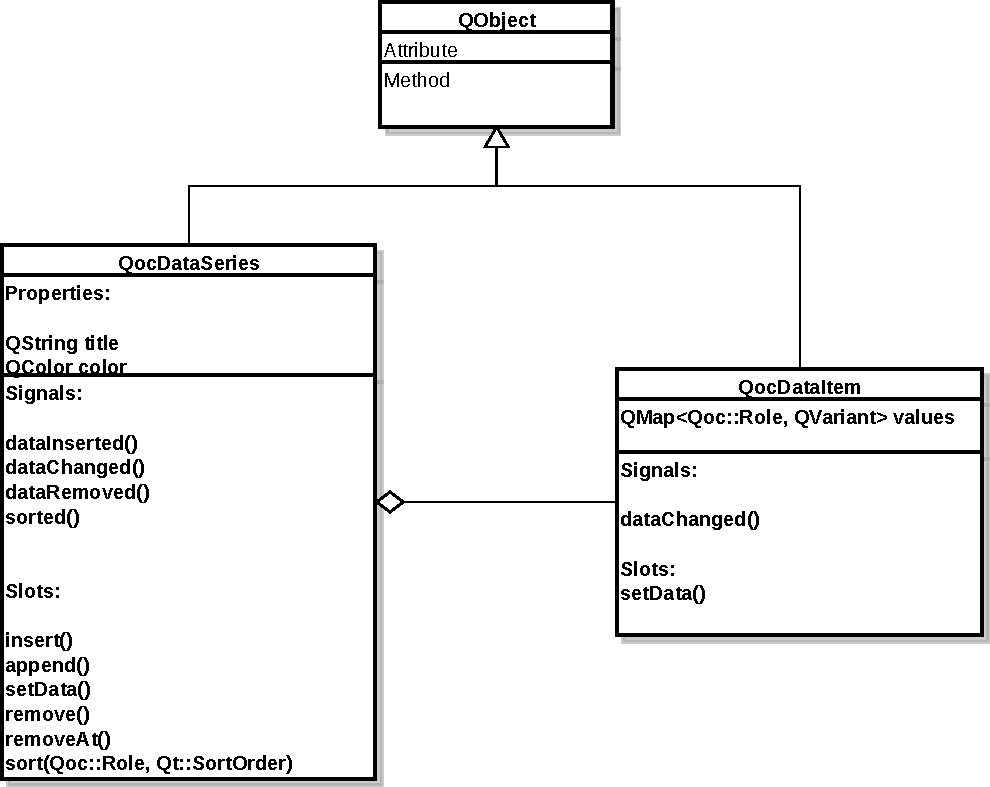
\includegraphics[scale=0.8]{img/seria_danych.pdf}
\caption{Seria i próbki}\label{rys:seria}
\end{figure}

\subsection{QAbstractItemModel}
Pracując na seriach danych, które są mojego autorstwa, mogę założyć, że dla elementu o~danym indeksie i~roli wartość jest, np. tytułem zapisanym w~łańcuchu znaków. Takiego komfortu jednak nie będzie przy współpracy z~dowolnym innym modelem. Nie mogę wymagać od użytkownika, aby interesujące mnie dane trzymał w~kolumnach o~ustalonych przeze mnie indeksach. Rozwiązaniem tej sytuacji mogłoby być stworzenie specjalnego proxy modelu~\footnote{Proxy modele \url{http://qt-project.org/doc/qt-5.0/qtcore/qabstractproxymodel.html}}, jednak preferuję inny sposób.

Moje rozwiązanie polega na mapowaniu ról, które są zrozumiałe dla wykresów, na numery kolumn modeli do tych wykresów podłączanych. W~przypadku jednowymiarowych modeli dziedziczących po \textit{QAbstractListModel} role wykresu będą mapowane na role tychże modeli. Z~perspektywy programisty mapowanie powinno się ograniczać jedynie do wywołania poniższej metody dla wszystkich wymagających tego ról:

\begin{verbatim}
QocAbstractChart::
setRoleMapping(Qoc::Role role, int customValue);
\end{verbatim}

Metoda ta przyjmuje jako pierwszy z~argumentów rolę, a~jako drugi numer kolumny, pod którą kryją się odpowiednie dane w~modelu.


\subsection{QML}
ListModel i XmlListModel to pochodne \textit{QAbstractListModel}, które należy potraktować osobno. Wprowadzają one bardziej obiektowe podejście, dzięki czemu ich zawartość jest łatwo dostępna z~QML.

Dane z~tych modeli są dostępne również poprzez system właściwości. Aby dostać się do wartości właściwości wystarczy jedynie znać jej nazwę. Dzięki temu, wymuszając na użytkownikach określone nazwy właściwości, jestem w~stanie pobierać dane z~ich modeli. W~skrajnym przypadku, gdy programista korzystający z~mojej biblioteki nie będzie mógł dostarczyć danych w~oczekiwanym przeze mnie formacie, udostępniam mu przeładowaną metodę z~poprzedniego podpunktu:

\begin{verbatim}
QocAbstractChart::
setRoleMapping(Qoc::Role role, const QString &name);
\end{verbatim}

W~tym przypadku jako drugi argument przyjmuję nową nazwę danej właściwości. Po wywołaniu metody, nowa nazwa właściwości będzie wykorzystywana do komunikacji z~modelem.


\section{Qt Quick}
Wykorzystanie mojej biblioteki w~Qt~Quick wymaga pewnego narzutu pracy. Poniżej opisuję mechanizm umożliwiający wykorzystanie moich klas w~QML oraz przyjętą przeze mnie konwencję interfejsów dla QML.

\subsection{Eksport klas C++ do QML}
Klasy wszystkich wysokopoziomowych elementów powinny być pochodnymi klasy QObject. Wszelkie ich parametry, które powinny być konfigurowane przez programistów należy włączyć do zbioru właściwości tej klasy. W~szczególności należy zadbać o~to, aby przy zmianie wartości danej właściwości, i~tylko wtedy, emitować sygnał informujący o~tym zdarzeniu. Jest to niezbędne do poprawnego działania mechanizmu wiązania w~QML. Ponadto, wszystkie metody, które powinny być dostępne z~QML, a~nie są slotami, powinny zostać opatrzone makrem \textit{Q\_INVOKABLE}.

Większość klas powinna być gotowa do wyeksportowania ich do QML za pomocą standardowej procedury, np. poprzez wywołanie funkcji szablonowej
\begin{verbatim}
template<typename T>
int qmlRegisterType(const char *uri, int versionMajor, 
		    int versionMinor, const char *qmlName)
\end{verbatim}
Parametrem szablonu jest eksportowany typ, a~parametry funkcji to nazwa modułu, dwie liczby odpowiadające za wersję modułu oraz nazwa pod jaką będzie dostępna eksportowana klasa z~poziomu QML. Qt udostępnia jeszcze kilka innych, specjalizowanych szablonów, np. dla singletonów.

Pozostałe klasy, do wykorzystania ich w~QML, będą wymagały specjalnych interfejsów. Dla klas związanych z~GUI, bazujących na QPainter będzie to QQuickPaintedItem, a~dla tych wykorzystujących SceneGraph -- QQuickItem.

\subsection{Uproszczony interfejs}
Aby zapobiec nadmiernemu rozrostowi interfejsów klas dostępnych w~QML, zdecydowałem się je uprościć w~porównaniu do tych dostępnych z~poziomu C++. Jest to konwencja szeroko stosowana w~QML. Najlepszym przykładem będzie ramka wokół prostokąta. Z~poziomu C++ istnieje możliwość ustawienia pióra używanego do jej odrysowania. Klasa pióra, czyli \textit{QPen}, nie dziedziczy po \textit{QObject}, więc nie może być dostępna w~QML. W~QML można zmienić jedynie kolor oraz grubość ramki.

\section{Interaktywność}
Wszystkie operacje interaktywne zostały rozwiązane za pomocą systemu zdarzeń Qt~\footnote{System zdarzeń Qt \url{http://qt-project.org/doc/qt-5.0/qtcore/eventsandfilters.html}}. Widoki mają obowiązek przekazywać wszelkie przeznaczone dla wykresu zdarzenia, np. pojawienie się kursora myszy nad wykresem czy kliknięcie.

\subsection{Zaznaczanie}
Aby zrealizować zaznaczanie elementów wykresu z~poziomu GUI, do wykresu musza być przekazywane zdarzenia związane z~kursorem myszy oraz dotykiem. Pojedyncze kliknięcie w~element reprezentujący dane będzie skutkować jego zaznaczeniem. Podwójne kliknięcie takiego elementu spowoduje zaznaczenie wszystkich elementów danej serii. Zaznaczenie powoduje zmianę koloru obramowania wokół danego elementu. Kolor zaznaczenia jest zdefiniowany jako właściwość całego wykresu.

\subsection{Zmiana wartości w modelu}
Na rysunku~\ref{rys:seq:inter} przedstawiam diagram sekwencji dotyczący zmiany zawartości modelu poprzez modyfikację elementów widoku. Przerywane strzałki zawierające opis symbolizują wywołanie sygnału.

\begin{figure}[H]
\centering
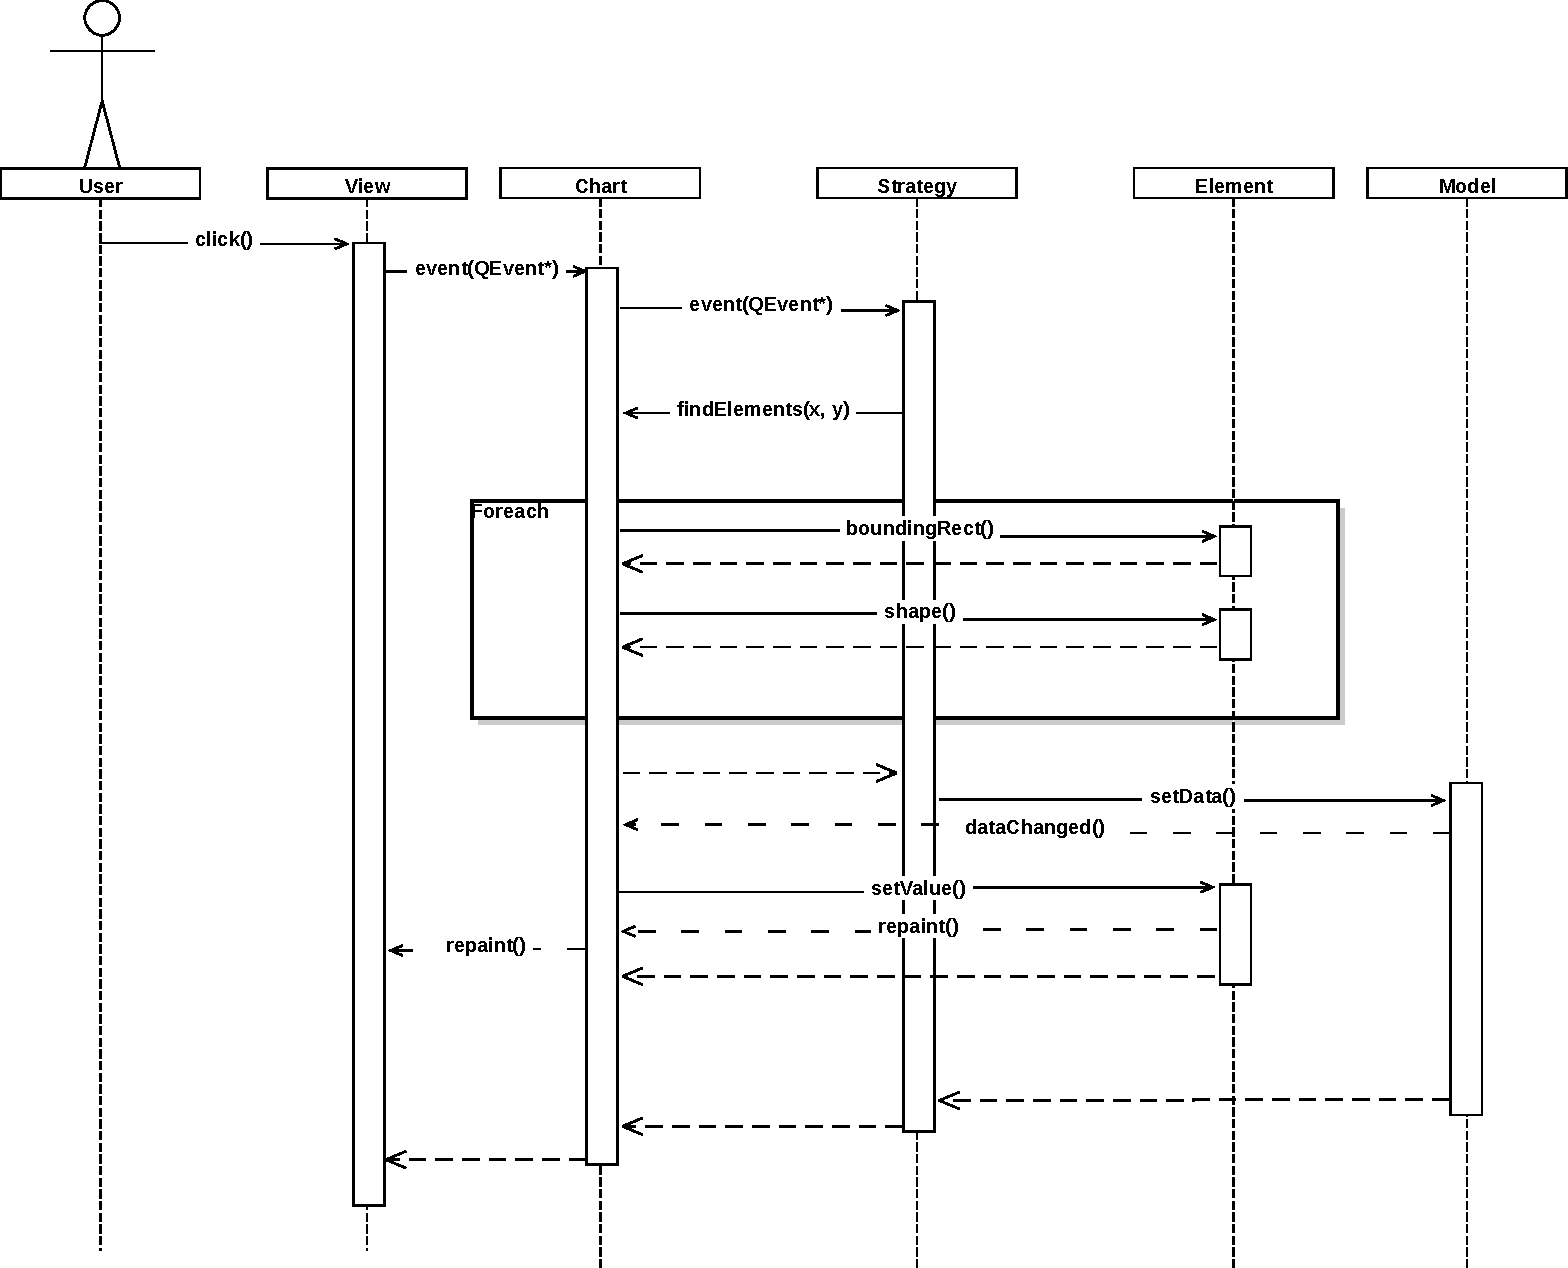
\includegraphics[scale=0.6]{img/seq_inter.pdf}
\caption{Interaktywna zmiana zawartości modelu}\label{rys:seq:inter}
\end{figure}

\section{Wykresy w układzie współrzędnych}
Większość wykresów jest osadzona w~pewnym układzie współrzędnych. Najpopularniejszym z~nich jest układ współrzędnych kartezjańskich~\ref{rys:uk:kart}, jednak jak wiadomo nie jest to jedyny układ współrzędnych. Moje rozwiązanie przewiduje możliwość tworzenia wykresów w~bardziej egzotycznych układach, np. wykres polarny w~układzie biegunowym~\ref{rys:uk:bieg}.

Mimo, iż najpopularniejszą skalą osi, stosowaną przy wykresach biurowych jest skala liniowa, moje rozwiązanie przewiduje możliwość wykorzystania innej skali, np. logarytmicznej, która jest dość często stosowana przy wykresach liniowych. 

\begin{figure}[H]
\centering
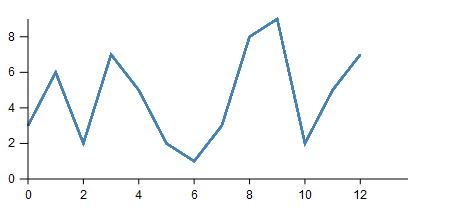
\includegraphics[scale=0.65]{img/kartezjanski.png}
\caption{Liniowy wykres w układzie kartezjańskim}\label{rys:uk:kart}
\end{figure}

\begin{figure}[H]
\centering
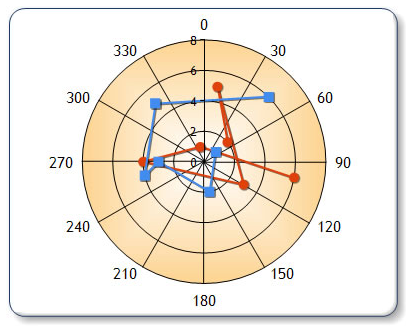
\includegraphics[scale=0.65]{img/biegunowy.png}
\caption{Wykres polarny}\label{rys:uk:bieg}
\end{figure}

Na diagramie~\ref{rys:os:skala} prezentuję hierarchię klas związanych z~układem współrzędnych. Jedyną klasą nie przewidzianą do dziedziczenia jest tu \textit{QocAxis}. Pozostałe elementy tej hierarchi powinny być dostosowywane do własnych potrzeb poprzez dziedziczenie.

\begin{figure}[H]
\centering
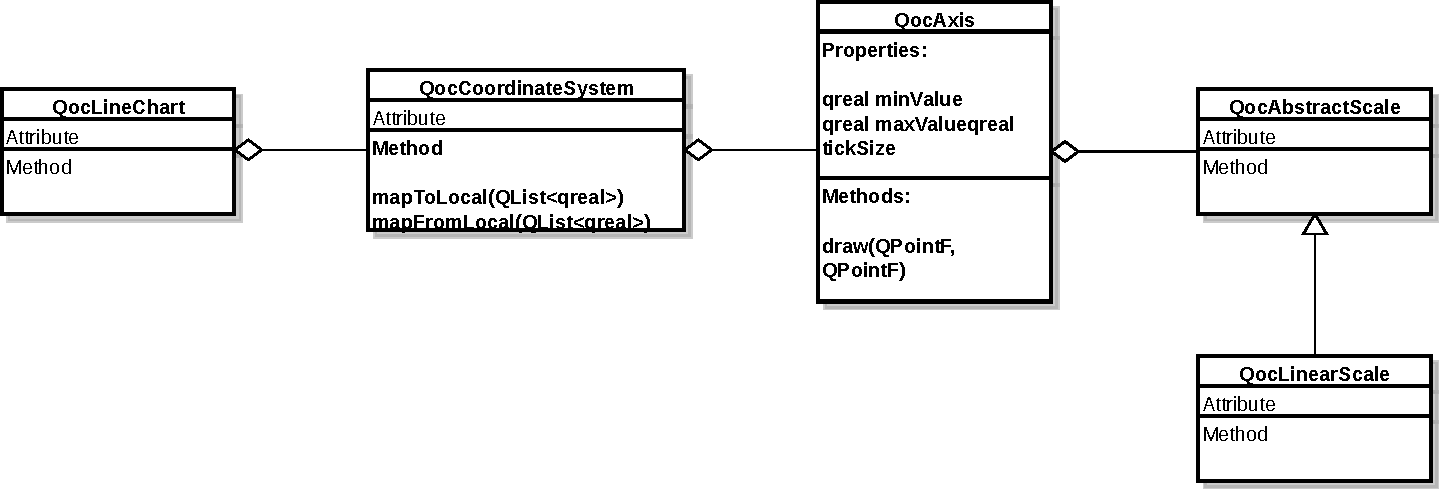
\includegraphics[scale=0.5]{img/os_skala.pdf}
\caption{Klasy związane z układem współrzędnych}\label{rys:os:skala}
\end{figure}

\subsection{Układ współrzędnych}
,,Układ współrzędnych -- funkcja przypisująca każdemu punktowi danej przestrzeni (w szczególności przestrzeni dwuwymiarowej -- płaszczyzny, powierzchni kuli itp.) skończony ciąg (krotkę) liczb rzeczywistych zwanych współrzędnymi punktu.''~\footnote{\url{http://pl.wikipedia.org/wiki/Układ\_współrzędnych}}

Głównym celem istnienia bytu o~nazwie \textit{QocAbstractCoordinateSystem} jest udostępnienie dwóch funkcji. Pierwsza z~nich przyjmuje wektor opisujący położenie punktu w~danej przestrzeni i~zwraca dwie współrzędne -- x~i~y tego punktu na płaszczyźnie wykresu. Druga funkcja działa dokładnie dokładnie odwrotnie. Takie podejście powinno umożliwić dwukierunkowe mapowanie przestrzeni dwuwymiarowych, ale może być niewystarczające dla wykresów 3D. 

Poza wyżej opisaną funkcjonalnością układ współrzędnych odpowiada w~mojej bibliotece również za zarządzanie osiami oraz odrysowywanie siatki. Wydzielenie takiego bytu jak układ współrzędych umożliwi jego współdzielenie między różnymi wykresami.

\subsection{Osie i skale} 
Według mnie oś w układzie współrzędnych powinna być możliwie prostą i~niezmienną klasą, dlatego postanowiłem rozłączyć oś od jej skali -- jest to rozwiązanie podobne do zastosowanego w~Qwt~\footnote{Skala w Qwt \url{http://qwt.sourceforge.net/class\_qwt\_scale\_engine.html}}. Oś jest odpowiedzialna głównie za swoje odrysowywanie, pozostałe zadania związane z~wyliczaniem współrzędnych czy ticków oddelegowuje do swojej skali. Domyślną skalą jest skala liniowa, ale takie podejście umożliwia włączenie do biblioteki, np. skali logarytmicznej.

\section{Legenda}
Legenda jest elementem służącym do prezentacji dwóch właściwości: koloru oraz tytułu. W~zależności od typu wykresu są to właściwości pojedynczej próbki albo całej serii. 

Dodawanie legendy do wykresu odbywa się za pomocą metody \textit{QocAbstractChart::setLegend()}, która podłącza sygnały płynące ze źródła danych do obiektu klasy \textit{QocSignalMapper}. Zmapowane sygnały są podłączane do odpowiednich slotów legendy. Za pomocą specjalnego typu wyliczeniowego da się sparametryzować czy mapowanie ma zostać dokonane dla pojedynczych próbek czy dla całych serii. Cała koncepcja została zobrazowana na diagramie~\ref{rys:diag:legenda}.

\begin{figure}[H]
\centering
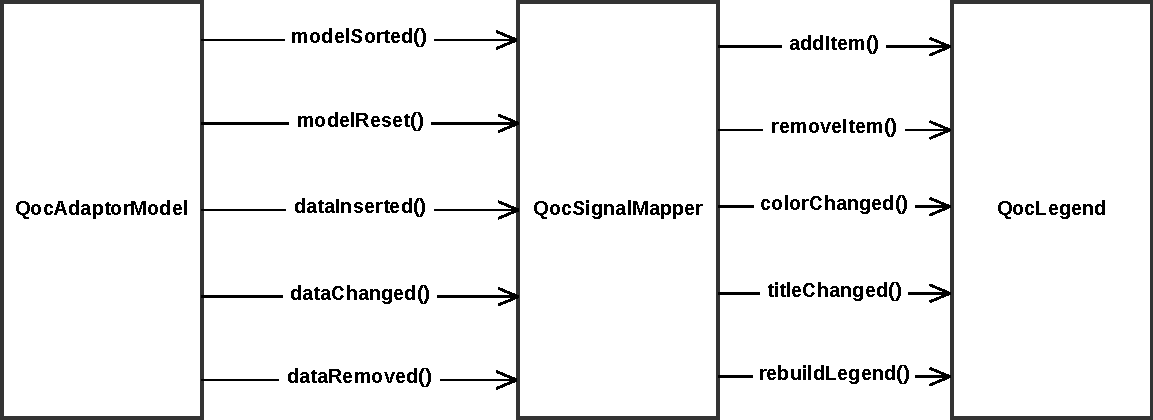
\includegraphics[scale=0.7]{img/legenda.pdf}
\caption{Komunikacja pomiędzy źródłem danych a legendą}\label{rys:diag:legenda}
\end{figure}

\subsection{Delegat}
Możliwość zmieny elementu prezentującego w~legendzie kolor rozwiązałem przez dodanie nowej właściwości legendy -- delegata. Musi to być obiekt klasy dziedziczącej po \textit{QObject}. Klasa ta musi posiadać metodę \textit{draw()}, jeśli korzysta z~\textit{QPainter}, albo \textit{updatePaintNode()} dla \textit{SceneGraph}. Podczas odrysowywania legendy będę wywoływałe jedną z~tych metod korzystając z~systemu metadanych Qt -- wykorzystam metodę \textit{QMetaObject::invokeMethod()}. Do tworzenia kolejnych instancji delegata wykorzystam metodę \textit{QMetaObject::newInstance()}.  Dodatkowo delegat musi mieć właściwość kolor. Spełnienie tych kilku warunków sprawi, że programista będzie mógł wyświetlić w~legendzie kwadrat, trójkąt albo kwiatek. Domyślny delegat to element o~kształcie kwadratu.

\section{Współpraca wykresów z widokami }
Jak już zostało ustalone, celem tworzonej biblioteki jest stworzenie uniwersalnego silnika, umożliwiającego tworzenie wykresów gotowych do podpięcia do jednego z~kilku widoków. Na rysunku~\ref{rys:widok:wykres} przedstawiłem składniki protokołu komunikacji między widokiem a dowolnym wykresem z~mojej biblioteki.

Widok ma obowiązek przesyłać do wykresu wszelkie zdarzenia, które są dla niego przeznaczone oraz informować wykres o~zmianach swojej geometrii. Ponadto przy odrysowywaniu widok musi wywoływać metodę \textit{draw()} wykresu.

Wykres nie powinien posiadać informacji z~widokiem jakiej klasy współpracuje. Można to osiągnać za pomocą mechanizmu sygnałów i~slotów, który pozwala na luźne wiązanie elementów. Odpowiednie sygnały  powinny być emitowane przez wykres zawsze wtedy, gdy wymaga on ponownego odrysowania.
Sygnał \textit{repaint()} powinien być emitowany w~sytuacji gdy ponowne odrysowanie musi nastąpić niemal natychmiast, natomiast sygnał \textit{update()} jest przeznaczony na sytuacje gdy zgłoszenia odrysowania mogą zostać skolejkowane, sklejone i~obsłużone jako jedno zgłoszenie w~najbliższej wolnej chwili.


\begin{figure}[H]
\centering
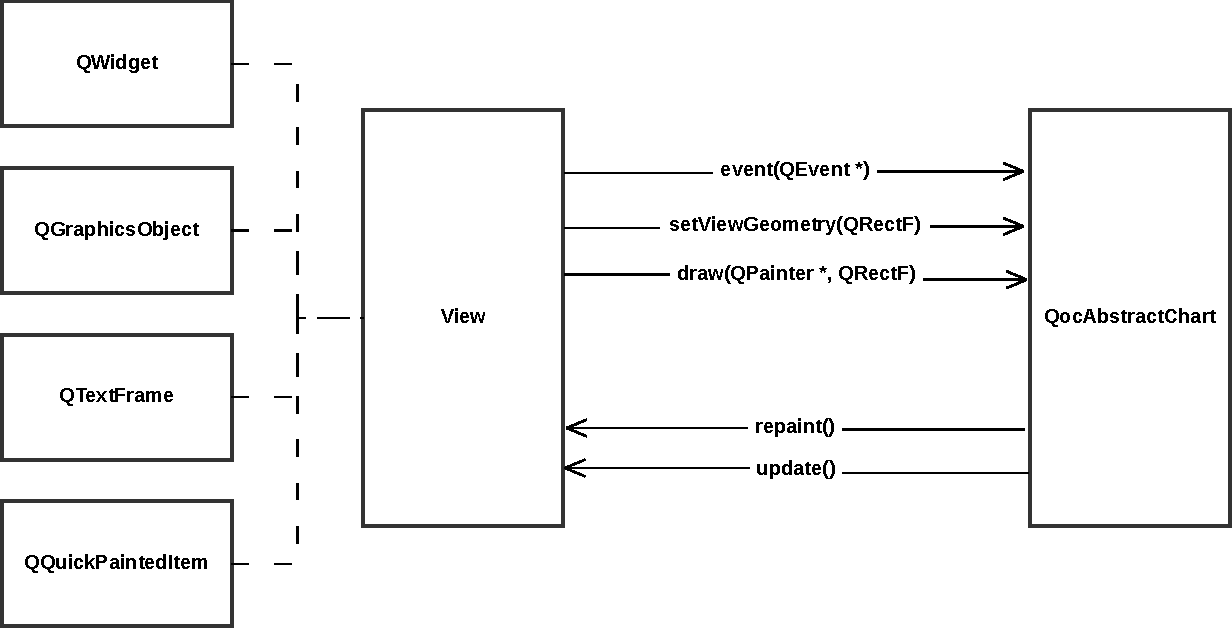
\includegraphics[scale=0.75]{img/widok-wykres.pdf}
\caption{Widok -- Wykres}\label{rys:widok:wykres}
\end{figure}

%\subsubsection{Wskazówki implementacyjne}
%Klasa bazowa wykresów powinna posiadać właściwość typu prostokąt, opisującą geometrię widoku podłączonego do danego wykresu. Zmiana tej właściwości powinna się odbywać poprzez odpowiedni slot, przyjmujący jako argument nowy prostokąt.

%W~zależności od klasy, z~której wywodzi się widok podłączony do wykresu, slot powiadamiający wykres o~zmianie geometrii widoku powinien być wywoływany następujących metodach widoku:
%\begin{itemize}
%\item{QWidget}
%	\begin{itemize}
%	\item{moveEvent()}
%	\item{resizeEvent()}
%	\end{itemize}
%\item{QGraphicsObject}
%	\begin{itemize}
%	\item{prepareGeometryChange()}
%	\end{itemize}
%\item{QTextFrame}

%\item{QQuickPaintedItem}
%	\begin{itemize}
%	\item{geometryChanged()}
%	\end{itemize}
%\end{itemize}

\section{Zależności między plikami}
Mogłoby się wydawać, że każde nowe wydanie Qt powinno wymagać ponownej kompilacji projektów zeń korzystających. Tak jednak nie jest. Twórcy Qt zadbali o~to, aby zawsze wtedy, kiedy to możliwe, zachowana była zgodność binarna. Oznacza to, że jeśli przy poprawkach do nowej wersji nie zostały zmienione nagłówki klas, a~jedynie ich implementacje, to przebudowanie całej aplikacji nie jest konieczne. Teoretycznie przejście z~Qt~w~wersji 4.8.3 na wersję 4.8.4 może odbyć się jedynie poprzez podmianę plików .dll. Temat zgodności binarnej oraz zależności czasu kompilacji między plikami został poruszony przez Scotta Meyersa~\cite{50Ways}.

\subsection{QObject}
Klasa QObject została zaprojektowana jako \textit{Most}~\cite{Patterns}.
%, zmodyfikowany o~posiadany przez ciało wskaźnik do uchwytu. 
Podział na uchwyt i~ciało zmniejsza zależności pomiędzy plikami bibliotek Qt i~znacząco skraca czas kompilacji po zmianach w~kodzie. Dodatkowo QObject posiada konstruktor przyjmujący jako argument wskaźnik do ciała, dzięki czemu można je zaalokować tylko raz, w~klasie najniższego poziomu hierarchii dziedziczenia, a~następnie przekazać jako argument konstruktora klasy bazowej. 
Koncepcję \textit{Mostu} zobrazowałem w~kontekście mojej biblioteki na rys.~\ref{rys:dpointer}.\newline

\begin{figure}[H]
\centering
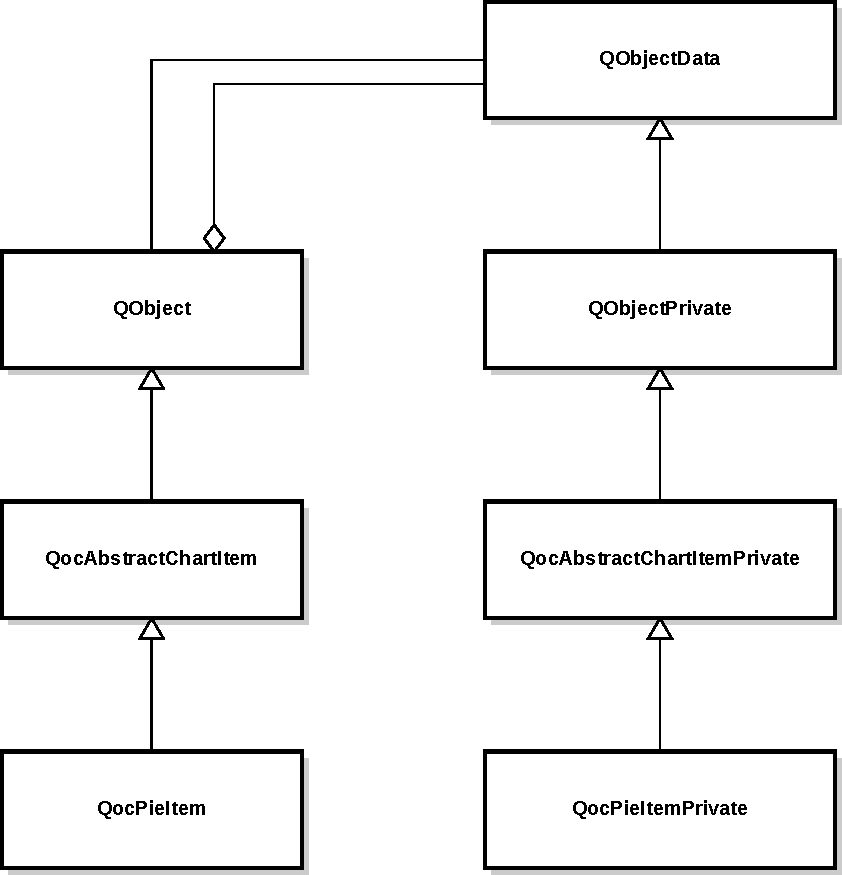
\includegraphics[scale=0.8]{img/dpointer.pdf}
\caption{Przykładowa hierarchia klas}\label{rys:dpointer}
\end{figure}

W~Qt przyjęto następującą koncepcję nazewniczą:
\begin{itemize}
\item{uchwyt ma standardową nazwę, zgodną ze swoim przeznaczeniem,}
\item{ciało ma nazwę składającą się z~nazwy odpowiadającego mu uchwytu oraz sufiksu ,,Private''.}
\end{itemize}


\subsection{Dostęp do uchwytów i ciał}
Podejście opisane w~poprzednim punkcie skutkuje jednak powstaniem pewnego efektu ubocznego.
Wskaźniki do uchwytu i~ciała są typów klas znajdujących się na szczycie hierarchii dziedziczenia. Dostęp do metod klas pochodnych niewystępujących w~klasach bazowych wymaga rzutowania w~dół. 
Problem ten rozwiązano za pomocą czterech makrodefinicji przyjmujących jako argument nazwę klasy uchwytu. Dwie z~nich należy wywołać w~odpowiednich nagłówkach. Z~kolei pozostałe dwie należy wywoływać na początku każdej metody wymagającej odwołania do ciała lub uchwytu. Miejsce wykorzystania konkretnych makr podaję w~tablicy~\ref{tab:makra}. Technika ta została szczegółowo opisana w~artykule~\footnote{QObject -- Most \url{http://qt-project.org/wiki/Dpointer}}.

\begin{table}[h]\footnotesize
\centering
\caption{Makrodefinicje}
\label{tab:makra}
\begin{tabular}{|c|c|c|}
\hline
Miejsce & Uchwyt & Ciało\\
\hline
Nagłówek & Q\_DECLARE\_PRIVATE & Q\_DECLARE\_PUBLIC\\
\hline
Metoda & Q\_D & Q\_Q\\
\hline
\end{tabular}
\end{table}

\chapter{Implementacja}
Podczas pracowni dyplomowej nie miałem wiele czasu na implementację biblioteki. Udało mi się wykonać jedynie prototyp rozwiązania w~postaci uproszczonego wykresu słupkowego. Jest to rozwiązanie niepełne, które jednak implementuje najważniejsze mechanizmy z~rozdziału \textit{Projekt}~\ref{chap:proj}. 

Poniżej opisuję narzędzia, które wykorzystałem podczas prac nad biblioteką. Następnie opisuję najciekawsze szczegóły implementacyjne oraz odstępstwa od projektu. Na koniec przedstawiam zaimplementowany przeze mnie wykres słupkowy.

\section{Wykorzystane narzędzia}
Do stworzenia tej pracy inżynierskiej wykorzystałem najlepiej znane mi narzędzia. Ze wszystkich opisanych poniżej, tylko Qt~5 było dla mnie pewną nowością. Z~pozostałych korzystam zarówno w~pracy, jak i~na uczelni.
 
\subsubsection{Qt 5}
Najnowsza dostępna wersja Qt to 5.1. Nowa odsłona dostarcza programistom szereg usprawnień oraz modułów, m.in. do obsługi formatu JSON. Jednak głównym punktem Qt~5 jest nowa implementacja Qt~Quick. 

Do implementacji Qt~Quick~2 wykorzystano OpenGL i~SceneGraph, co znacznie poprawiło wydajność tego systemu. Qt~5 rozpoczęło też nowy kierunek rozwoju aplikacji wykorzystujących Qt. Qt~Quick jest promowany jako zalecany sposób tworzenia interfejsów użytkownika. Docelowo aplikacje Qt mają być podzielone na GUI napisane w~QML oraz logikę zaprogramowaną w~C++.

\subsubsection{Qt Creator}
Qt~Creator to zintegrowane środowisko programistyczne przeznaczone głównie dla języków C++, QML oraz JavaScript. Jego edytor tekstowy zawiera takie udogodnienia jak kolorowanie składni czy narzędzia do refaktoryzacji kodu. Qt~Creator zawiera także wtyczkę do tworzenia graficznych interfejsów użytkownika. Korzystanie z~Designera jest proste i~intuicyjne, a~proste GUI można w~dużej mierze ,,wyklikać''.

Do budowania i~debugowania Qt~Creator wykorzystuje domyślne oprogramowanie danej platformy, np. kompilator gcc i~debuger gdb na systemie Linux. Creator posiada graficzny interfejs do debuggera, który w~znaczący sposób upraszcza procesz debugowania.

Qt~Creator posiada również wtyczki integrujące go z~najpopularniejszymi systemami kontroli wersji. Lista wspieranych systemów:
\begin{itemize}
\item{Bazaar,}
\item{CVS,}
\item{Git,}
\item{Mercurial,}
\item{Perforce,}
\item{Subversion.}
\end{itemize}

\subsubsection{Subversion}
Subversion to scentralizowany system kontroli wersji będący następcą systemu CVS. Repozytorium SVN założyłem w~serwisie Google Code~\footnote{http://code.google.com/intl/pl/}, pod adresem \url{http://code.google.com/p/qt-west-charts/}.

\subsubsection{Kubuntu 12.04 LTS}
Kubuntu to pochodna Ubuntu, korzystająca z~KDE -- graficznego środowiska, zbudowanego w~oparciu o~bibliteki Qt. ,,Kubuntu oznacza \textit{w stronę ludzkości} w języku bemba''~\footnote{Kubuntu \url{http://pl.wikipedia.org/wiki/Kubuntu}} -- jest to cytat, który jednoznacznie wskazuje co jest celem istnienia tej dystrybucji Linuxa.

Kubuntu jest udostępniane z~bogatym zbiorem aplikacji biurowych, multimedialnych oraz wielu innych. Najpopularniejsze aplikacje, które są dostarczane wraz z~systemem Kubuntu to LibreOffice i~GIMP. 


\section{Szczegóły implementacyjne}
Rozdział \textit{Projekt}~\ref{chap:proj} nie jest bardzo precyzyjną dokumentacją techniczną. Celem tego rozdziału było przedstawienie pewnych rozwiązań architektonicznych, których uszczegółowienie było możliwe dopiero na etapie implementacji, gdyż jako projektant, nie byłem w~stanie przewidzieć wszystkich trudności związanych z~implementacją. Ten podrozdział służy uszczegółowieniu pewnych kwestii, które dotychczas nie zostały wystarczająco rozwinięte.

\subsection{Nieidealna separacja}
W mojej bibliotece odseparowałem warstwę prezentacji od warstwy danych poprzez podział na wykres oraz model. Wykres odpowiada za prezentację danych, których źródłem jest model. Dany model może być źródłem danych dla wielu wykresów.

Separacja tych dwóch warstw nie jest jednak idealna, gdyż model zawiera takie informacje jak kolor czy tytuł próbki. Uniemożliwia to zaprezentowanie tych samych danych w~dwóch wykresach za pomocą różnych palet kolorów. Podejście to ma jednak swoje plusy. Sprawia, że użytkownik nie musi ,,zaglądać'' do wewnętrznych elementów wykresu. Stworzenie prostego wykresu ogranicza się do powołania jego instancji i~podłączenia źródła wypełnionego danymi. Taka prostota jest szczególnie porządana w~przypadku deklaratywnego języka, jakim jest QML.

Na myśl przyszło mi kilka rozwiązań tego problemu, ale wydają mi się one albo niezbyt eleganckie, albo nazbyt skomplikowane. Zdaje się, że najwłaściwszym byłoby wprowadzenie elementu takiego jak delegat~\footnote{Delegat \url{http://qt-project.org/doc/qt-5.0/qtwidgets/model-view-\newline programming.html\#delegates}} w~architekturze \textit{Model-Widok}. Byłoby to odpowiednie rozwiązanie dla doświadczonych programistów, chcących tworzyć bardziej zaawansowane wykresy.

Z uwagi na prostotę użycia zdecydowałem się pozostać przy obecnym rozwiązaniu. Jeśli wyżej opisany problem okaże się palący dla użytkowników, będę zmuszony wprowadzić mechanizm delegatów.

\subsection{Elastyczność źródła danych}\label{sub:flexible}
Dzięki zastosowaniu dwóch ciekawych technik programistycznych osiągnąłem bardzo dużą elastyczność przy wyborze źródła danych dla wykresu. Pierwsza z~nich, to przyjmowanie jako model obiektu \textit{QVariant}. Druga to wprowadzenie adptera modelu~\ref{sec:zrodla}, który jest mostem~\ref{sec:most}.

Dodanie nowego źródła danych ogarnicza się do zarejestrowania klasy źródła jako \textit{QVariant} oraz obsłużenia tego źródła w~ciele mostu. Uchwyt mostu pozostaje niezmieniony, dzięki czemu wprowadzenie nowego źródła danych nie spowoduje ponownej kompilacji całej biblioteki oraz aplikacji z~niej korzystajacych, a~jedynie ponowne linkowanie.

\subsection{Wtyczka Qt~Quick}
Rozszerzenia Qt~Quick są realizowane poprzez system wtyczek, które są ładowane na starcie aplikacji. Głównym celem takiej wtyczki jest zarejestrowanie wszystkich klas C++, które później mają być dostępne w~QML. Wtyczka musi dziedziczyć po klasie \textit{QQmlExtensionPlugin}, a~rejestrowane klasy muszą być pochodnymi \textit{QObject}.

W przypadku mojego projektu, wtyczka zawiera adaptery do klas biblioteki, realizujących właściwą funkcjonalność. Zdecydowałem się zastosować takie podejście z~kilku powodów.

Po pierwsze, nie wszystkie klasy Qt są dostępne z~poziomu QML. Najlepszym przykładem jest pędzel, czyli obiekt klasy \textit{QBrush}. Programiści C++ mają możliwość ustawienia wszystkich parametrów pędzla odpowiedzialnego za odmalowanie tła wykresu. Z~poziomu QML udostępniam możliwość ustawienia tylko koloru pędzla.

Kolejny argument przemawiający za moim rozwiązaniem, to uniknięcie przesadnie rozbudowanych interfejsów. Udostępnienie wszystkich parametrów pędzla za pomocą systemu właściwości spowodowałoby drastyczne rozbudowanie interfejsu danej klasy.

Ostatnim, przeważającym argumentem jest fakt, że właśnie takie podejście jest standardowym rozwiązaniem stosowanym przy eksponowaniu klas C++ do Qt~Quick. W~QML udostępniane są jedynie najważniejsze parametry, np. kolor pędzla, a~te mniej znaczące są pomijane. Wydruk~\ref{code:qoc:adapter} zawiera przykładowy adapter znajdujący się we wtyczce Qt~Quick mojej biblioteki.

\begin{lstlisting}[caption=Adapter klasy QocAbstractChart, label=code:qoc:adapter]
class QOC_QUICK_API QocQuickAbstractChart : public QocAbstractChart
{
	Q_OBJECT
	Q_PROPERTY(QColor backgroundColor 
		   READ backgroundColor 
		   WRITE setBackgroundColor 
		   NOTIFY backgroundColorChanged)
	...
}
\end{lstlisting}


\subsection{Biblioteka na platformie Windows}
Podczas budowania dowolnej biblioteki na platformie Windows, niezbędne jest wyeksportowanie symboli. Proces ten muszą przejść wszystkie elementy, które mają być dostępne dla klientów danej biblioteki. W~przypadku mojego projektu eksportowane były jedynie nagłówki klas, jednak mogą to być również globalne funkcje lub zmienne. Eksport symboli odbywa się za pomocą dostarczanych przez Qt makrodefinicji, których wykorzystanie w~mojej bibliotece przedstawiam na wydrukach~\ref{code:qoc:global} i~\ref{code:qoc:klasa}.

\begin{lstlisting}[caption=Zawartość pliku qoc\_global.h, label=code:qoc:global]
#include <QtCore/QtGlobal>

#if defined(QOC_LIBRARY)
#  define QOC_API Q_DECL_EXPORT
#else
#  define QOC_API Q_DECL_IMPORT
#endif
\end{lstlisting}

\begin{lstlisting}[caption=Eksport klasy QocAbstractChart, label=code:qoc:klasa]
#include "qoc_global.h"

class QOC_API QocAbstractChart : public QObject
{
   ...
}
\end{lstlisting}


Dzięki dodadniu do pliku projektu instrukcji: \textit{DEFINES +=  QOC\_LIBRARY}, podczas budowania biblioteki makro \textit{QOC\_API} powoduje wyeksportowanie symboli. Z~kolei dla klientów biblioteki makro po rozwinięciu przez preprocesor spowoduje ich import.


\section{Odstępstwa od projektu}
Faza implementacji zweryfikowała założenia projektowe. Część z~nich się obroniła, pozostałe musiałem nagiąć bądź całkowicie z~nich zrezygnować. Poniżej opisuję wszystkie sytuacje, w~których postępowałem niezgodnie z~projektem.

\subsection{Oszczędne korzystanie ze wzorca Most}
Zmniejszenie zależności między plikami poprzez wykorzystanie wzorca mostu, opisane w~rozdziale~\ref{sec:most}, dostarczyło mi dość dużo dodatkowej pracy. Dlatego postanowiłem korzystać z~tego rozwiązania jedynie tam, gdzie ma to sens.

Miejscami, w~których dodatkowa praca przeznaczona na stworzenie mostu się zwraca, są klasy przeznaczone do rozbudowywanie. Są to klasy bazowe takie jak \textit{QocAbstractChart} albo węzły takie jak \textit{QocAdaptorModel}. Korzyści wynikające z~zastosowania mostu w~takim miejscu opisałem w~punkcie~\ref{sub:flexible}. Natomiast proste klasy, które nie są przeznaczone do dziedziczenia, jak \textit{QocAxis}, nie zostały zaimplementowane jako most.


\section{Prototyp wykresu słupkowego}
Udało mi się zaimplementować rdzeń wykresu słupkowego. Z~uwagi na niewielką ilość czasu pominąłem niektóre rozwiązania architektoniczne, jednak zachowałem najważniejsze z~nich, takie jak separacja danych od prezentacji czy podział wykresu na warstwy. 

W~obecnym stanie, za pomocą wykresu słupkowego można prezentować dane tylko z~jednej serii. Możliwa jest animacja elementów wykresu. W~przykładowym programie zaanimowałem wysokość słupków. Wykres podpiąłem do dwóch widoków -- widgetu oraz elementu QML. Poniżej znajdują się zrzuty z~ekranu, prezentujące ten wykres. 

\begin{figure}[H]
\centering
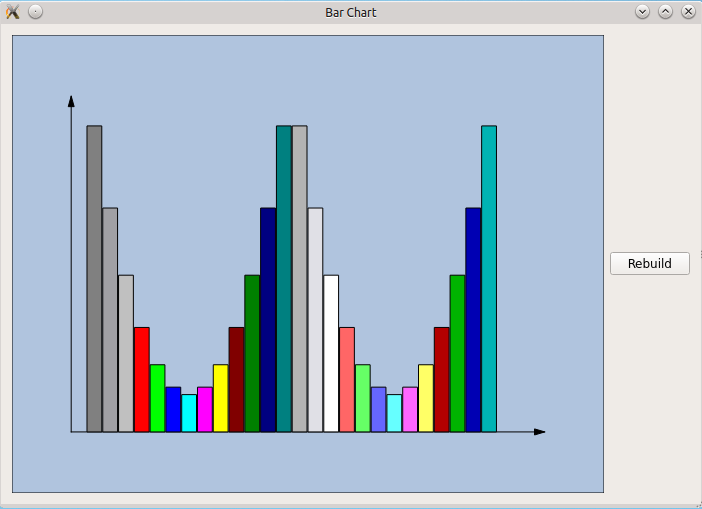
\includegraphics[scale=0.5]{img/BarChart_kubuntu.png}
\caption{Wykres słupkowy -- Kubuntu 12.04}\label{rys:bar:kubuntu}
\end{figure}

\begin{figure}[H]
\centering
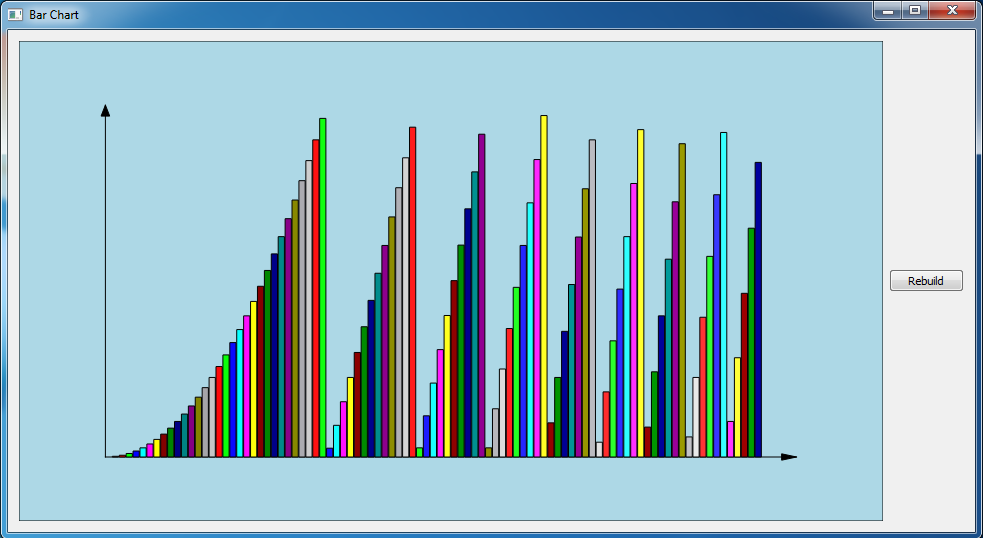
\includegraphics[scale=0.54]{img/BarChart_windows7.png}
\caption{Wykres słupkowy -- Windows 7}\label{rys:bar:windows7}
\end{figure}

%TODO: Windows 7 \& Qt~Quick

%\section{Tworzenie biblioteki współdzielonej}
%Biblioteka współdzielona to rodzaj biblioteki dynamicznej, czyli biblioteki łączonej z~programem dopiero w~trakcie jego uruchamiania. Przy pierwszym uruchomieniu programu korzystającego z~danej biblioteki współdzielonej, biblioteka ta zostaje załadowana w~całości do pamięci. Od tej pory wszystkie programy, będą mogły korzystać z~tej biblioteki bez ponownego jej ładowania. W~systemach Unixowych biblioteki dynamiczne mają rozszerzenie .so, a~w~systemach Windows .dll.

%Qt udostępnia nam stosunkowo prosty sposób na tworzenie bibliotek dynamicznych.

%\subsection{Symbole}
%Wszelkie funkcje, zmienne i klasy zawarte w~bibliotece, które są przeznaczone do użytku dla klientów biblioteki są nazywane publicznymi symbolami i~muszą zostać wyeksportowane, czyli upublicznione podczas kompilacji biblioteki. Zazwyczaj domyślne zachowanie kompilatorów to ukrywanie wszystkich symboli. Aby stały się one dostępne dla klientów biblioteki, trzeba to otwarcie zasygnalizować podczas kompilacji. Natomiast na niektórych platformach osobnych instrukcji wymaga ukrycie symboli.

%\subsection{Eksport -- Import}
%Rozwiązaniem obu problemów są dwa makra dostarczane przez Qt, które muszą zostać dodane do deklaracji symboli:
%\begin{itemize}
%\item{Q\_DECL\_EXPORT -- przy kompilacji dynamicznej biblioteki}
%\item{Q\_DECL\_IMPORT -- przy kompilacji klienta korzystającego z~biblioteki}
%\end{itemize}

%\subsection{Uniwersalne makro}
%Teraz trzeba się upewnić, że odpowiednie makro zostanie wykorzystane w~odpowiednim momencie. Typowym rozwiązaniem jest dodanie specjalnego pliku nagłówkowego, np. \textit{foolib\_global.h}. Plik ten musi zawierać kod preprocesora realizujący następującą sztuczkę:
%\begin{lstlisting}[caption=Warunkowa kompilacja, label=code:kompilacja:warunkowa]
%#include <QtCore/QtGlobal>

%#if defined(FOOLIB_LIBRARY)
%#  define FOOLIB_API Q_DECL_EXPORT
%#else
%#  define FOOLIB_API Q_DECL_IMPORT
%#endif
%\end{lstlisting}

%Jak widać, w~zależności od tego czy istnieje makro \textit{FOOLIB\_LIBRARY}, makro \textit{FOOLIB\_API} posłuży do eksportowania albo importowania symboli biblioteki \textit{FooLib}. Makro \textit{FOOLIB\_LIBRARY} zostanie zdefiniowane tylko i~wyłącznie w~pliku projektu biblioteki \textit{FooLib}. Tylko wtedy będziemy mieli pewność, że nasza biblioteka będzie poprawnie linkowana. W~pliku .pro należy dodać instrukcję: \textit{DEFINES +=  FOOLIB\_LIBRARY}.

%\subsection{Wykorzystanie makra}
%We wszystkich plikach nagłówkowych biblioteki, deklaracje symboli muszą zostać uzupełnione o~nasze makro:

%\begin{lstlisting}[caption=Eksport symboli, label=code:eksport:sym]
%#include "foolib_global.h"

%FOOLIB_API void foo();
%class FOOLIB_API Foo...
%\end{lstlisting}


\documentclass[11pt,twoside,a4paper,final]{article}
\usepackage[utf8]{inputenc}
\usepackage[T1]{fontenc}
\usepackage[MeX]{polski}
\usepackage{graphicx}
\usepackage{url}
\usepackage{hyperref}
\usepackage{listings}
\bibliographystyle{splncs}

\begin{document}

\date{28 lipca 2013}
\title{QTestLib \\}

\author{Łukasz Szewczyk}
\maketitle


\section{Wstęp}
W celu osiągnięcia kodu o~wysokiej jakości należy przeprowadzać jego testy. Jest to szczególnie ważne przy tworzeniu bibliotek, gdyż wszelkie błędy w~nich zawarte wpływają negatywnie na programy klientów.
Biblioteką odpowiedzialną za testy w~Qt jest QtTestLib~\cite{qtest}. Biblioteka ta udostępnia narzędznia umożliwiające pisanie testów jednostkowych, testów starowanych danymi oraz testów wydajnościowych. 

\section{Testy jednostkowe}
Poniżej opisuję kolejne kroki prowadzące do stworzenia zbioru testów jednostkowych w~Qt.

\subsection{Podstawa}
Podstawą tworzonych testów jednostkowych jest klasa, którą należy stworzyć. Musi ona dziedziczyć po QObject, a~wszystkie testy jednostkowe muszą być realizowane w~metodach tej klasy, z~kolei metody te muszą być prywatnymi slotami. Zabieg ten jest konieczny, aby QTestLib mógł wykryć wszystkie nasze funkcje testowe.

\subsection{Implementacja funkcji testowych}
Funkcje testowe są zazwyczaj prostymi kawałkami kodu, w~których sprawdzany jest efekt wywołania metody testowanej klasy. Jeśli jest on zgodny z~oczekiwaniami to test jest zaliczany i~system przechodzi do następnego testu. W~przeciwnym przypadku test jest oblewany, a~informacja o~tym zdarzeniu zostaje zapisana w~logu. W~zależności od ustawień aplikacj testowej, może ona zostać w~tym momencie przerwana, bądź kontynuowana do samego końca. 
QTestLib swoje funkcjonalności za pomocą zbioru makrodefinicji, przykłady:
\begin{itemize}
\item{QVERIFY(warunek) -- sprawdzenie bool-owskiej wartości. Prawda zalicza test.}
\item{QCOMPARE(faktyczna,~oczekiwana) -- porównanie dwóch wartości. Równość zalicza test.}
\end{itemize}

\subsection{Utworzenie funkcji main}
Utworzenie funkcji main naszego testu sprowadza się do wykorzystania makra, które jako argument przyjmuje nazwę naszej funkcji testowej, np.\newline 
\textit{QTEST\_MAIN(TestOfSomeClass)}. Tak utworzona funkcja main sprawi, że wszystkie nasze funkcje testowe zostaną uruchomione.

\subsection{Uruchomienie testu}
Aby zbudować naszą testową aplikację należy wpisać w~konsoli następujące komendy:
\begin{lstlisting}
qmake -project "CONFIG += qtestlib"
qmake
make
\end{lstlisting}

\section{Testy sterowane danymi}
Aby odseparować logikę testów od danych, którymi będą zasilane, należy utworzyć dla każdego testu dwa sloty:
\begin{lstlisting}
void someTest();
void someTest_data();
\end{lstlisting}
Pierwszy ze slotów odpowiada za test jednostkowy, natomiast drugi za dostarczenie danych do owego testu. Technika ta bardziej szczegółowo została omówiona w~artykule~\cite{datadriven}.
Zastosowanie w tym przypadku makra \textit{QTEST\_MAIN()} spowoduje uruchomienie każdego testu dla wszystkich przygotowanych dlań zestawów danych.

\section{Testy wydajnościowe}
Tworzenie testów wydajnościowych, czyli tzw. benchmark-ów, jest możliwe za pomocą makra \textit{QBENCHMARK}. Przykładowy test:
\begin{lstlisting}
void TestBenchmark::simpleTest()
{
	Foo foo;

	QVERIFY(foo.doSomething());

	QBENCHMARK 
	{
		foo.doSomething();
	}
}
\end{lstlisting}

Za pomocą tej techniki oraz testów sterowanych danymi można stworzyć automatyczne testy porównujące wydajność danego rozwiązania dla różnych zbiorów danych.

\section{Testy w mojej bibliotece}
Testy jednostkowe
Testy regresji


\begin{thebibliography}{}

\bibitem[1]{qtest}
Testy w Qt \url{http://qt-project.org/doc/qt-5.1/qttestlib/qtest-overview.html}
\bibitem[2]{datadriven}
Testy sterowane danymi \url{http://qt-project.org/doc/qt-4.8/qtestlib-tutorial2.html}


\end{thebibliography}

\end{document}

\chapter{Podsumowanie}

\section{Wnioski}

\section{Kierunki rozwoju}



\appendix

% tutaj załączniki

%\chapter*{Bibliografia}
\renewcommand{\bibname}{Spis literatury}
\nocite{*}
\bibliographystyle{plplain}
%\bibliographystylebk{plplain}
%\bibliographystylest{plplain}
%\bibliographystyledoc{plplain}
% \bibliographystyleweb{plplain}
%\bibliographybk{BIB/books}
%\bibliographyst{BIB/books}
%\bibliographydoc{BIB/books}
% \bibliographyweb{BIB/books}

% \bibliography{bib/verificard,bib/jml,bib/daikon}
\bibliography{bib/bibliografia}

\end{document}

% ex: set tabstop=4 shiftwidth=4 softtabstop=4 noexpandtab fileformat=unix filetype=tex spelllang=pl,en spell:

